\documentclass[12pt]{article}


\usepackage{setspace}
\doublespace
\usepackage{multicol}
\usepackage{parskip}
\usepackage{titlesec}
\usepackage[section]{placeins}
\usepackage{xcolor}
%\usepackage{breakcites}
\usepackage{lineno}
\usepackage{hyphenat}
\usepackage{CharisSIL}
\usepackage{pdflscape}






\PassOptionsToPackage{hyphens}{url}
\usepackage[colorlinks = true,
            linkcolor = blue,
            urlcolor  = blue,
            citecolor = blue,
            anchorcolor = blue]{hyperref}
\usepackage{etoolbox}
\makeatletter
\makeatother






\renewenvironment{abstract}
  {{\bfseries\noindent{\abstractname}\par\nobreak}\footnotesize}
  {\bigskip}

\titlespacing{\section}{0pt}{*3}{*1}
\titlespacing{\subsection}{0pt}{*2}{*0.5}
\titlespacing{\subsubsection}{0pt}{*1.5}{0pt}


\usepackage{authblk}


\usepackage{graphicx}
\usepackage[space]{grffile}
\usepackage{latexsym}
\usepackage{textcomp}
\usepackage{longtable}
\usepackage{tabulary}
\usepackage{booktabs,array,multirow}
\usepackage{amsfonts,amsmath,amssymb}
\providecommand\citet{\cite}
\providecommand\citep{\cite}
\providecommand\citealt{\cite}
\newif\iflatexml\latexmlfalse
\providecommand{\tightlist}{\setlength{\itemsep}{0pt}\setlength{\parskip}{0pt}}
\usepackage[utf8]{inputenc}



\usepackage{float}

\begin{document}

\title{not all oppositions are lost} 



\author[]{sally ransom}%
\affil[]{University of Texas at Austin}%


\vspace{-1em}



  \date{\today}


\begingroup
\let\center\flushleft
\let\endcenter\endflushleft
\maketitle
\endgroup


\bigskip
\begin{quote}\begin{center}
{\it I don't use folksongs, \\
folksongs use me}\\
-Veljo Tormis, Estonian composer and {\it regilaul} revitalist
\end{center}
\end{quote}


\titlepage





\sloppy







\section*{Abstract}

% This corpus phonetics study of Estonian folk songs examines vowel space and duration in conflict and concordance at the song and the syllable-levels of prosodic prominence. Songs are useful for examining acoustic correlates of stress because they are restricted in the domain of time, having less temporal variation than natural ``running" speech.\cite{ .} 
%
%By examining the interaction of temporal and spatial acoustic cues in various positions, we can see how a singer accommodates prosodic conflicts to preserve contrasts in the language. 
The paper first introduces prosodic prominence in general, then delves into the metrical specifics of Estonian and its folksong tradition. After outlining the research questions, the methods section describes the corpus of {\it regilaul} songs: its construction, annotation, and processing. Results show that for vowel duration, song position is the best predictor of vowel length p(<0.05), while both short (Q1) and overlong (Q3) vowels show significant (p< 0.05) temporal acommodations (i.e., the contrast is retained at the segmental, not the syllabic level, where the vowel in the overlong is shortened to make space for the additional consonants) to the note duration at level of the song. Both song and syllable stress showed a significant increase in vowel space (p<0.05).  
\section*{Introduction}

\begin{itemize}
\item Cognitive science research in music and language: papers 
\item speech and singing: tone langs, melodic contours...
\item remaining questions
\end{itemize} 

At the cognitive interface of language and music are lyrical songs and songwriting traditions, where natural language participates in the musical domain as the resonator for the vocal instrument in sung and spoken languages is the same resonator used to make utterances. The speaking apparatus, a human wind instrument, is parasitic on the respiratory system \cite{ , }. To sing does not require language (i.e., lilting, yodeling) but incorporating words requires only some adjustments to timbre ( i.e., singing an /i/ sound instead of an open /a/), rhythm (accommodating the beats of a lyrical phrase into the musical meter of the song, or dividing a measure into enough notes for all the words, to impose meaningful utterances over a sung melody. Many lyrical songwriting traditions make use of repeated patterns\cite{ , }: be it lines or couplets of the same pattern in verses, or simpler refrains which alternate between larger groups of repeated material (verses). This repetition often results in a consistent duration rate for a relative phrasal isochrony throughout. Running speech, on the other hand, is not so isochronous \cite{, }. In this domain we can examine the effects of the musical context on the language, particularly with regards to temporal aspects. While bpm varies naturally in human singing, phrases in musical contexts are more consistent than in running speech \cite{,}. This paper takes the interface of music and language as an opportunity for an exploratory corpus phonetics study of syllable prominence using the Estonian language, which has three syllable quantities, a predictable stress pattern at the word level and a robust tradition of folksongs {\it regilaul} which follow a strict metrical pattern. We ask: what happens, acoustically, when meaningful linguistic utterance is fit into the metrical domain of its song's melody? 



\subsection*{Syllable Quantity \& Stress in Estonian} 

Estonian's stress system 

understanding of the quantity system is necessary to describe the stress system: 

\subsubsection{Estonian Quantity Degrees} 


Estonian has three quantities, resulting in three types of durationally contrastive feet, so that the same bisyllabic sequence can mean three different things depending on the quantity. 
 \begin{figure}[htbp]
 \begin{center}
 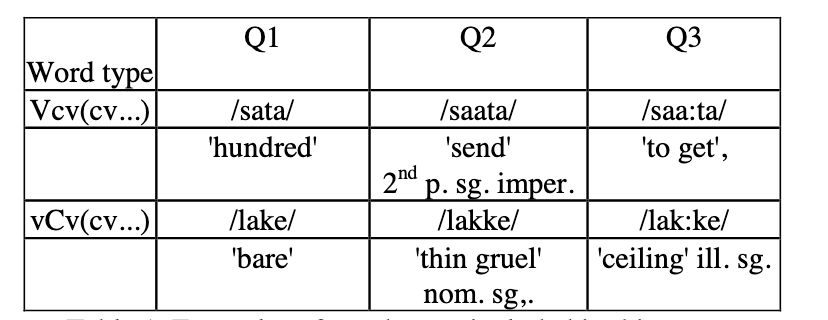
\includegraphics[width=200pt]{figures/Quantity.png}\\

 \caption{Three Way Quantity Contrast {\cite{traunmullerEffectLocalSpeaking2003}}}
 \label{quant_cont}
 \end{center}
 \end{figure}
 %(\it Krull, 1999)
 
 To describe the mechanisms of Estonian quantity contrast, it is necessary to understand both syllables and feet, as the ternary contrast is in proportional relation to the other members of its constituent\cite{lehisteProsodicChangeProgress2003}. 
 There is a documented tendency for foot isochrony \cite{ foxDiscriminationDurationRatios1987,foxDiscriminationDurationRatios1989, lehisteFunctionQuantityFinnish1965}, a consistency in duration of feet in Estonian which results in an inverse relationship between the durations of the two syllables in a foot: the longer the first syllable, the shorter the second. This is realized acoustically by the duration ratio of first and second syllable in a foot, i.e., second syllables that follow an overlong syllable will be realized shorter than a second syllable that follows a long syllable. \\
 \begin{enumerate}
 	\item Q1 – short 		ratio ~2/3	(short-long(er))
	\item Q2 – long		ratio ~3/2	(long(er)-short(er))
	\item Q3 – overlong		ratio ~2/1 	(long(er)-short(er)) 
\end{enumerate}

%  In list reading speech, the duration ratio is greater between short and long syllables, but in conversational speech this is only seen in situations where the bearer of quantity contrast is a vowel, and f0 is available as a secondary cue for quantity. In conversational speech when the contrast bearer is a consonant, the duration ratio is greater between long and overlong syllables. 

\subsubsection*{Stress in Estonian} 
 With few exceptions, such as in borrowed words, Estonian stress is predictable from the following rules:
 \begin{itemize}
 	\item if the syllable is in the third quantity, primary stress falls on its nucleus. 
	\item otherwise, primary word stress is on the first syllable. 
\end{itemize}
When a third-degree syllable is not in the first position, primary stress falls on it: this usually happens in the case of borrowed words. \cite{lehisteFunctionQuantityFinnish1965}. 


Estonian's stress is roughly trochaic, with main stress falling on the first syllable, and secondary stress falling iteratively on odd-numbered syllables counting from the left edge. When a third-degree syllable is not in the first position, primary stress falls on it: this usually happens in the case of borrowed words. \cite{lehisteFunctionQuantityFinnish1965}. 
In other words, a left-edge, quantity sensitive, iterative stress pattern.

\subsubsubsection*{Acoustic Correlates of Estonian Stress}
 Stress in Estonian is acoustically most often realized by onset consonant lengthening \cite{gordonPHONETICCORRELATESSTRESS1997} 
\subsection*{Kalevala Meter}
  The Kalevala meter is part of the musical tradition of both Estonia and Finland. The main element in the structure of the songs is the verse line, consisting of eight positions divided between four (usually trochaic) feet. From the point of view of musical rhythm, the majority of old folksong melodic phrases  (verse lines) are roughly isochronous, i.e. consisting of notes of about the same
 duration to about the same total phrase duration. In most cases, each of the eight positions holds one syllable for one melody note. As an exception, two syllables may fit one note, or a syllable (usually a diphthong) may be divided between two notes. This is readily evident in the musical score, which is divided into four or eight. Ictus refers to a position that is stressed in a song, and off-ictus is an unstressed position in a song. In {\it regilaul} songs, which make use of the Kalevala meter, the pattern is trochaic: ictus starts on the first beat and is applied to every other syllable of a phrase. \\
 
 
 \begin{figure}[htbp]
\begin{center}

\includegraphics[width=300pt]{melody.png}
\caption{one {\it regilaul} phrase in music notation}
\label{default}
\end{center}
\end{figure}


\subsubsubsection*{Perception of Estonian Stress} 


\subsection*{Previous Work}


  A previous study in Estonian \cite{rossTradeoffQuantityStress1996} found that duration was a better predictor of musical verse position than of word stress: stressed syllables in off-ictus lost their durational contrast with unstressed syllables.


 Another study, \cite{rossLostProsodicOppositions1994} compared S1/S2 ratios for all three quantity degrees in three Estonian funeral laments, finding that duration was best predicted by metrical position and not syllable quantity. 
In \cite{rossTimingEstonianFolk1998, rossTradeoffQuantityStress1996}, Ross and Lehiste measure syllable duration ratios (S1/S2) for two categories of Q1 initial syllables of diphones: falling in ictus position (stress concord) and falling in off-ctus position (stress conflict). They found that the duration ratios of Q1 syllables in ictus were greater than those in off-ictus (conflict). In initial position, Q1 syllables were roughly the same length as each other, while those in off-ictus were shortened. Thus the duration cue for contrastive stress is lost in the song. 
This paper aims to extend findings of the aforementioned studies of these songs' prosodic hierarchies by annotating a larger corpus of {\it regilaul}, to compare measurements of syllable duration ratios and proportional duration differences of syllable quantity and prominence in songs. By automating the annotation and measurement process using open source tools, the author hopes to share these machines with those who have similar research interests, and also to invite contributors to the data of this corpus of text data time-aligned to queryable audio signal data.  

If it is the case that duration contrasts are lost for syllable stress and quantity when put into songs, does any evidence of quantity and stress contrast remain in the signal? 
%
%%If not, then, accurate interpretation of the lyrics by the listener relies more heavily on contextual lexical information, i.e., syntactic structure, semantic context, pragmatics of the song as a whole as the acoustic information is more minimal. 
%
% If duration is subordinated to the prosody of the music, we can predict that another cue to linguistic stress will be retained in the singer’s production: for this paper, we will look at vowel quality. 






\subsection*{Research Questions and Hypotheses}

In languages which utilize stress systems, a syllable's prominence is indicated not by a single cue but by a convergence of several cues: i.e.,  duration\cite{dejongStressLexicalFocus2004}, spectral balance\cite{sluijterSpectralBalanceAcoustic1996}, vowel space\cite{dejongSupraglottalArticulationProminence1995}, onset consonant length \cite{gordonPHONETICCORRELATESSTRESS1997}, and can be thought of as localized hyperarticulation. \cite{libermanStressLinguisticRhythm1977},\cite{berinsteinWPPNo471979,}. 
Musical constituents also utilize rhythmic prominence, sometimes called `accented,' `'emphasized,' `strong,' all describing a proportional relation to other members of its constituents (i.e., a single note is a constituent, as are the notes in a measure,  the measures in a phrase, the phrase in its stanza, the whole song . \cite{}

Vowel duration, if subordinated to the song position, would confirm Ross \& Lehiste's results \cite{rossLostProsodicOppositions1994, rossTimingEstonianFolk1998, rossTradeoffQuantityStress1996} as any changes to the syllable overall (what they measured) would be ``to scale." Because consonant duration plays an important role in both stress and quantity in English, to see nuclei changing at a different rate than the consonant portions would indicate a reshuffling of the proportional ratio of segments within the syllable. 


Vowel Duration predictions: \\
words
\begin{itemize}
	\item null: the song level completely dominates the temporal domain:  there is no relationship 			between vowel duration and word-level duration contrasts. 	
	\item h 1: word-level duration contrasts will be preserved at the segmental level.
\end{itemize}
Vowel Space predictions: \\
If the domain of vowel space is shared, then both stress and ictus positions will have larger vowel spaces compared to their respective weaker neighbors. If the cue is not shared, it could be utilized by either ictus or by stress. Vowel space is essentially a manipulation of timbre, so, while a broader resonator can be used as a cue to a strong beat in a song, it doesn't conflict with the things that are most important to the song level: i.e., fundamental frequency and duration of the note being sung. So, vowel space as localized hyperarticulation could be an available cue to the word-level stress to utilize to maintain its contrast when duration is unavailable. \\
\begin{itemize}
	\item null : there is no relationship between vowel space and prominence in {\it regilaul} songs
	\item h2 : there is a relationship between vowel space and prominence in {\it regilaul} songs
		\begin{itemize}
		\item 2a : 	vowel space will be shared at both song and word levels of prominence
		\item 2b : vowel space best predicts word stress (S/w)
		\item 2c : vowel space best predicts song position (S/w)
		\end{itemize}
\end{itemize}
\section*{Methods}
In order to investigate these questions, a corpus of {\it regilaul} songs is assembled. 


\subsection*{Materials}

The Anthology of Estonian Traditional Music\cite{tampereAnthologyEstonianTraditional} provides an online overview of the folk music tradition of Estonia.  Along with the audio recordings, there are extensive supplementary materials: photographs and biographical information about the singers and musicians, lyrics (with English translations) of 98 {\it regilaul} songs and 17 instrumental tunes.

Originally published in on vinyl in 1970, later on compact disc in 2003, and finally  online as of 2016. The compilation showcases a sample of audio recordings of traditional {\it regilaul} collected by foklorists Herbert Tampere, Erna Tampere, and Ottilie Kõiva between 1912 and 1966 for the Estonian Folklore Archives in Tartu, Estonia. \\
For this project, a sample of 17 {\it regilaul} songs were selected to analyze, all recorded in Pärnumaa county between 1960 and  `65. 
 In this sample, seven women  ages between 67 and 92 (avg 75) years
 performers are seven women singing songs from their childhoods, passed down from previous generations, and some of their original compositions in the {\it regilaul} form.  At present, the corpus contains thirty-two minutes and twelve seconds of sung audio.

\subsection*{Preparing Audio and text} 
Files from the archive are losslessly converted with sox \cite{SoXSoundExchange} from .ogg to a .wav container.\footnote{: the conversion is lossless, necessitated due to the null bytes contained in .ogg files: the .wav format simply encodes null bytes as silence, increasing file size but enabling PRAAT\cite{boersnaPraatDoingPhonetics2022} to read the file.} Each song's lyrics are copied from the site and saved as .txt files in Estonian orthography (UTF-16), with each phrase (where a phrase is the text content for one measure of the song) separated by a new line. 
\subsubsection*{Beat Detection and Ictus Position} 
A given {\it regilaul} verse line contains eight beats, generally evenly divided into a single measure so that each of the eight syllables corresponds with one eighth note. The ictus position of a song's line is thus determinable by counting every other beat as ictus, starting with the first. There is natural tempo variation in singing, so in order to correctly determine ictus by position, both the position (rate) of each beat and the length (duration) of each beat need to accommodate these changes. For this, a tempo map is made using the Nyquist beat detective plugin \cite{AudioNyqNyquistAudacity}, the open source audio editor Audacity(R) \cite{Audacity}. The threshold is set so that wherein a note is labeled as a potential beat if it is 25\% more prominent (defined by the algorithm) than the surrounding acoustic signal (and fits into the detected overall tempo). The labels are adjusted to ensure that the downbeat of the song is annotated properly, and beats within measures are aligned at onset and containing the requisite number (usually four) of strong beats according to the music annotation.  The tempo map is then used as a guide for a MIDI instrument track, set to synchronize with the fluctuations in the song's tempo as documented by the map. Each note of the MIDI track is set to the appropriate duration for its note: i.e., for a typical series of eight eighth notes and eight syllables, four eighth notes are synthesized per verse measure on the `strong' beats. A script designed to mark silences and sounding portions of audio is run over the MIDI song, marking note containing (``sounding") intervals as ``ictus" and everything else as ``off." The resulting TextGrid fits the audio track of the song, and is used as the scaffolding for the for the remaining annotation tiers. 

\begin{figure}[htbp]
\begin{center}
			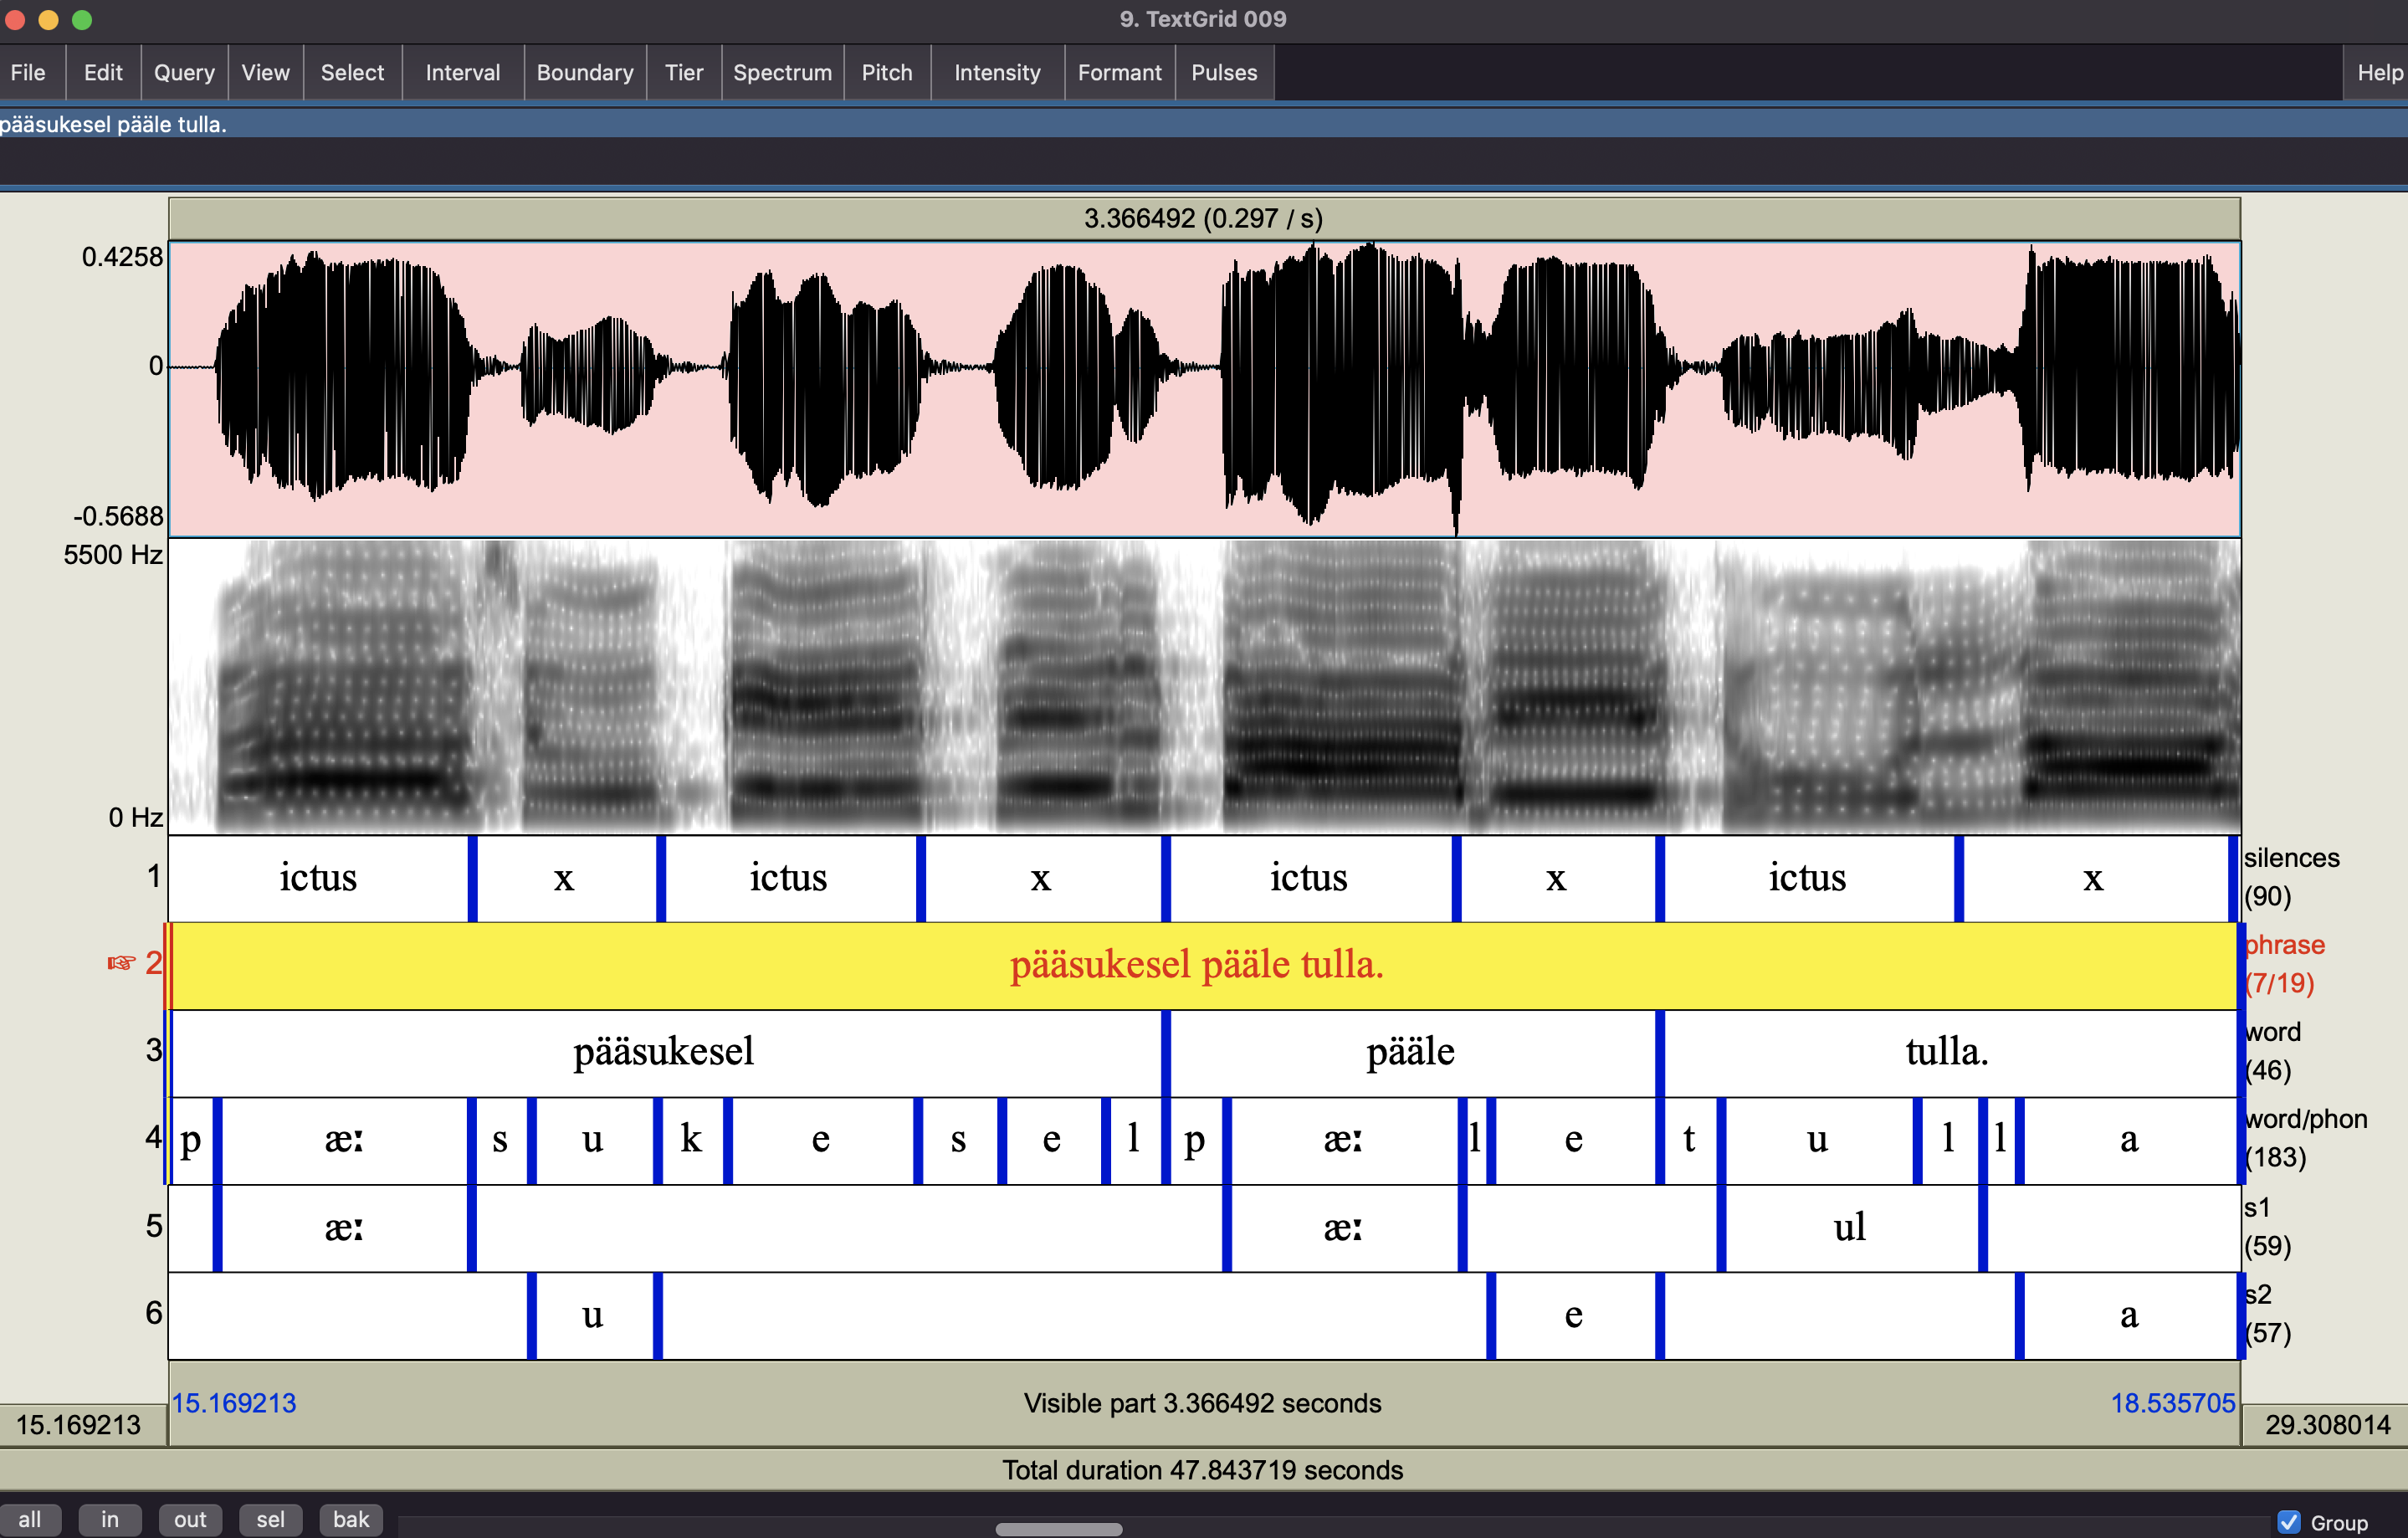
\includegraphics[width=300pt]{figures/phrase_grid.png}
			\caption{single phrase annotation}
\label{phrase}
\end{center}
\end{figure}

To annotate the phrases, the song's average bpm is divided by the number of lines in the song starting from the onset of the first ictus beat. The text files of the lyrics are then automatically inserted into each phrase interval. This is manually checked, and this tier also notes refrain and other portions to be excluded from the present analysis. Once each phrase interval has its appropriate lyrics, PRAAT's built-in eSpeak forced-aligner for Estonian is run on each phrase. eSpeak \cite{ESpeakSpeechSynthesizer} is an open source text-to-speech synthesizer. In PRAAT, these models can be used to synthesize Estonian speech from some annotation text, which is then  compared to the time-aligned audio signal and aligns the phonological transcription to the specified level(s), here both word and segment. Most often errors arise when a given word or segment is longer than the synthesizer expected (on account of being sung). In these situations, the word level tier is realigned so that it contains all and only the transcribed word, and then the forced aligner is re-run on this word to the segmental level. Intervals at the phoneme level are rarely edited after alignment except by deleting boundaries between non-identical vowels adjacent vowels  and vowels adjacent liquids, to all be analyzed as diphthongs. Long identical vowel boundaries are placed at the midpoint for duration measurement. 

\begin{figure}[htbp]
		\begin{center}
			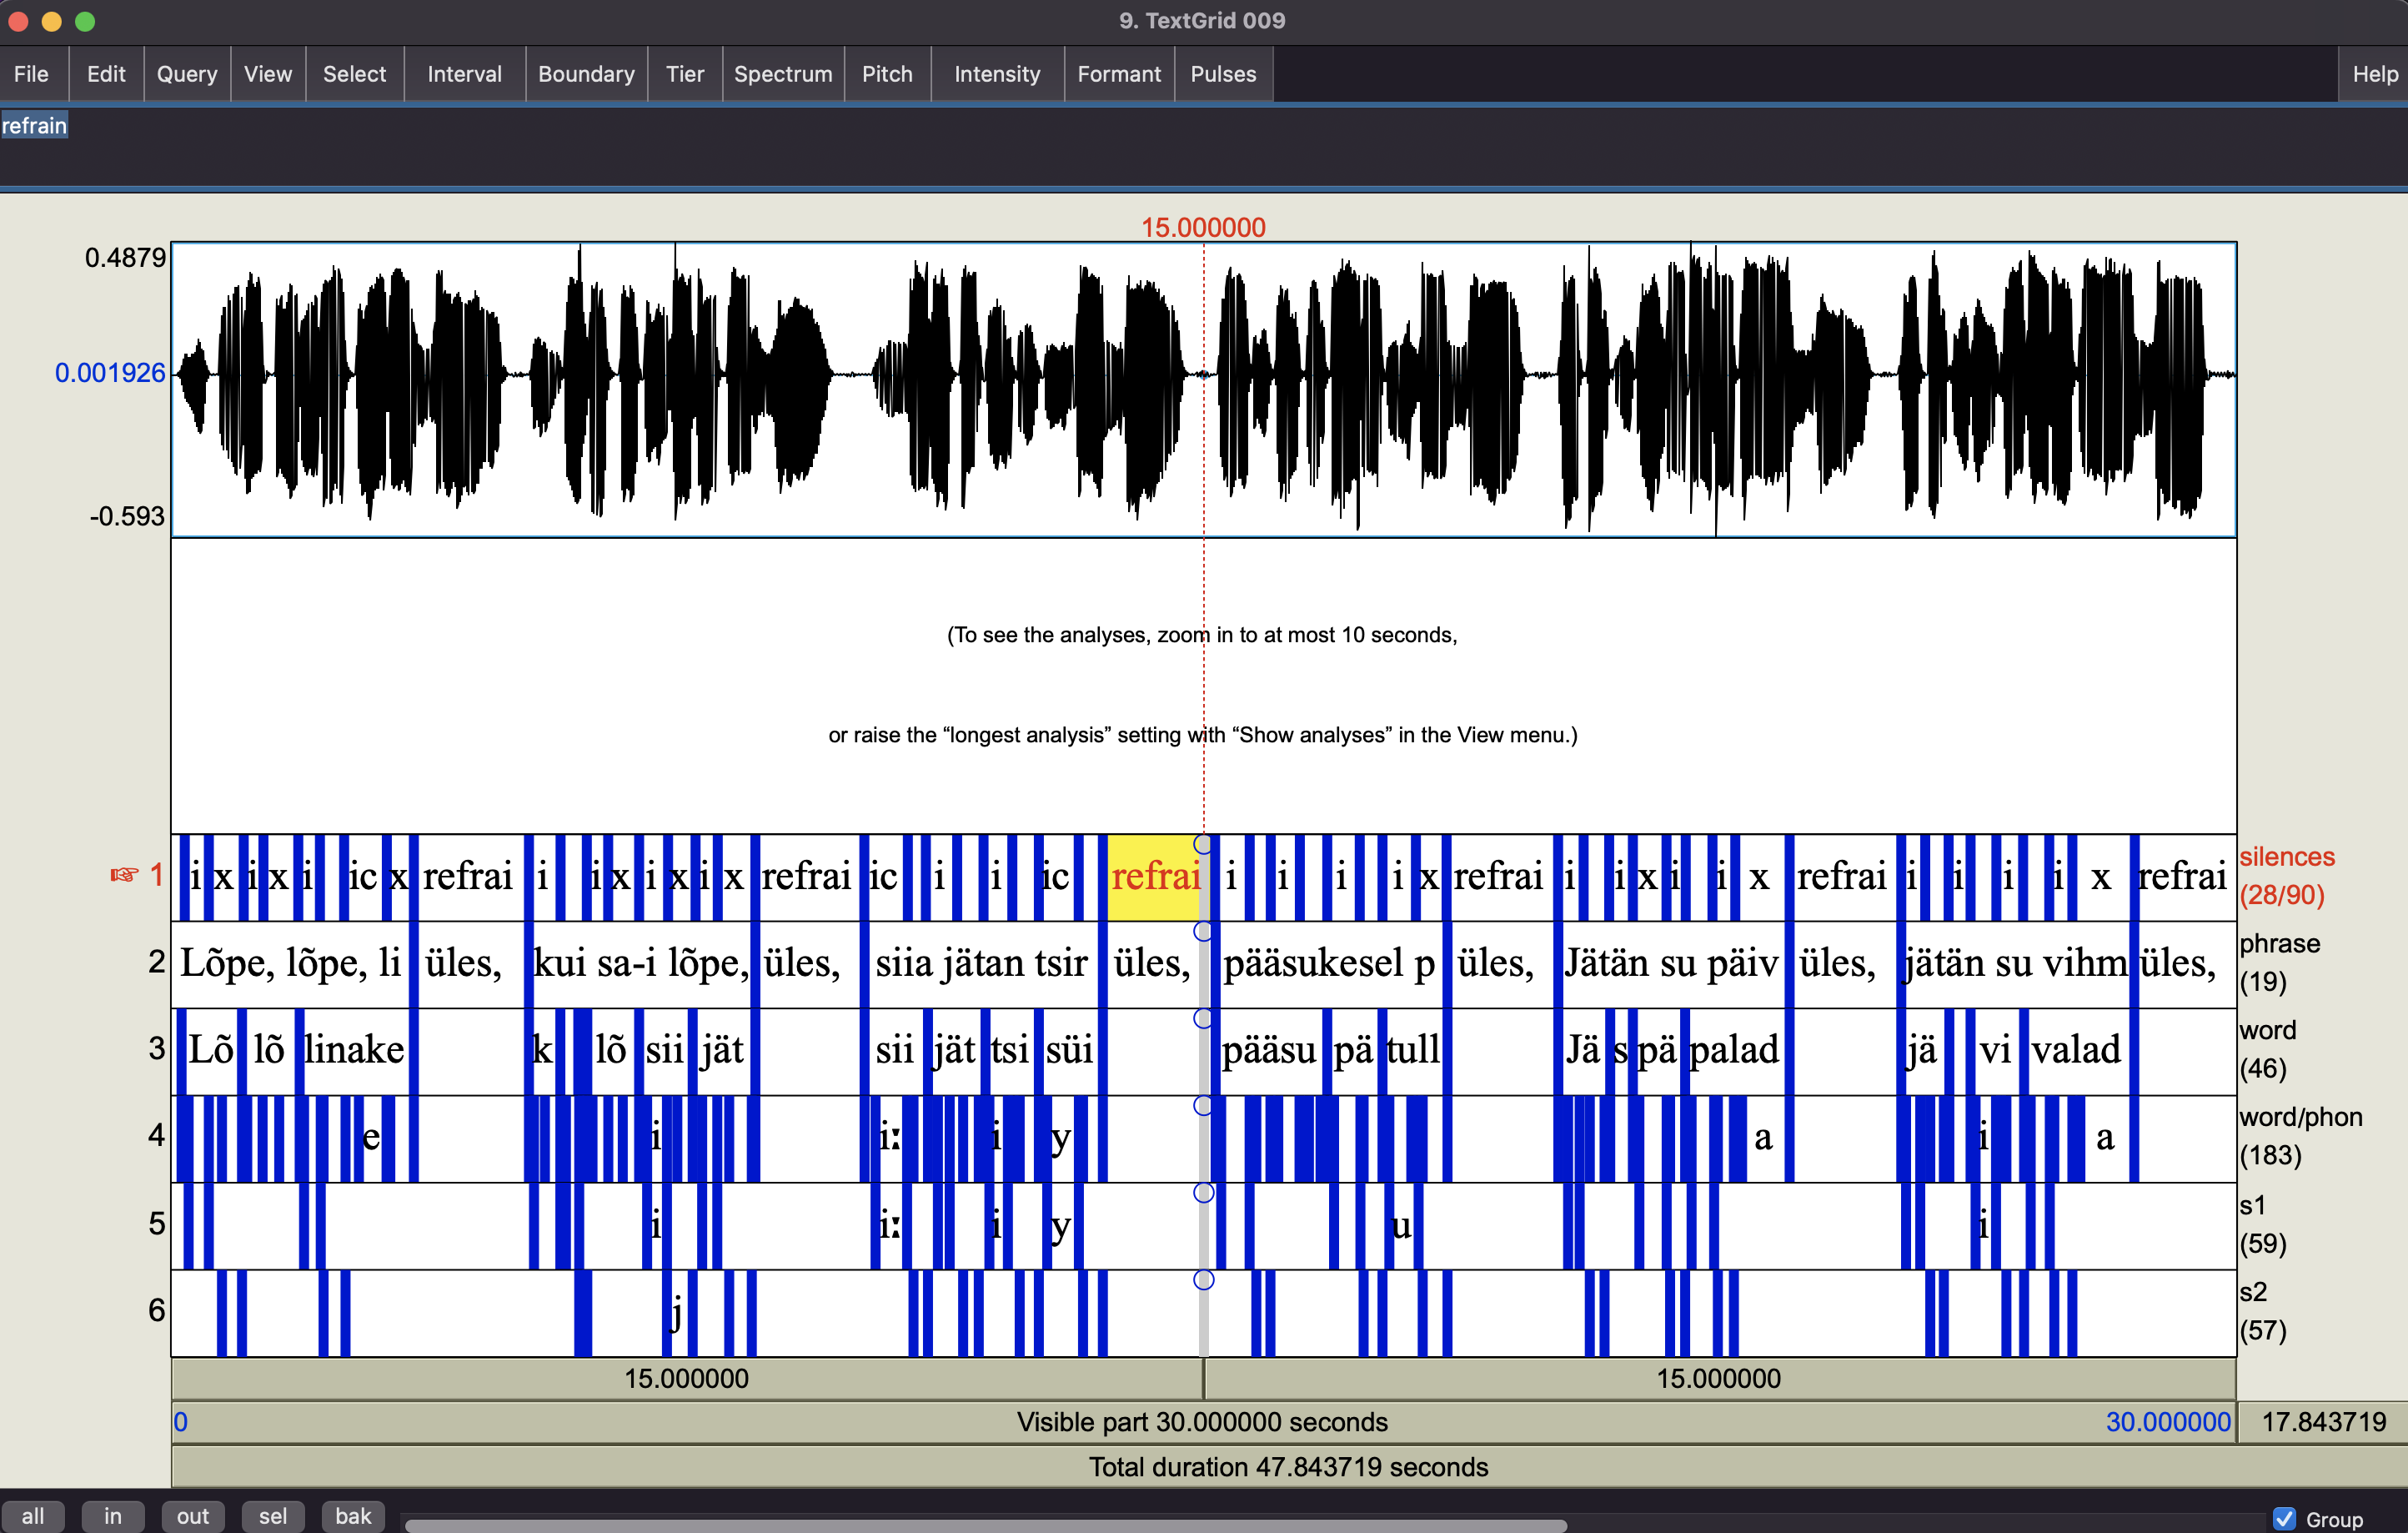
\includegraphics[width=300pt]{figures/big_grid.png}
			
			\caption{whole song annotation}
			\label{song_whole}
		\end{center}
\end{figure}
	
\subsection*{Text and Data Processing}

The lyrical text of each song is aggregated into a corpus of songs together with annotated and transcribed audio. Using estnltk's Estonian toolkit, text data is used to filter and sort the acoustic data by quantity, syllable boundary, syllable-word index (i.e. stressed or not in speech) and syllable-phrase index (ictus or not at this metrical position in the song). 

\subsubsection*{Varbamorf Syllabification}

At this point, the corpus is annotated for metrical position, phrase, word, and segment. Quantity contrasts, particularly Q2 and Q3, are not always obvious from the orthography. Thus, a syllable quantity and stress annotation are necessary. Using an estonian natural language toolkit has an automatic syllabifier library called ``varbamorf." The output of the syllabification in this module includes syllable quantity and prominence data as well as the phoneme segments in each respective syllable. 
%With the quantity annotated, duration measurements between syllable quantities can be compared with each other, to see if results are similar to \cite{rossTradeoffQuantityStress1996}.\\
%%


%\url{https://github.com/estnltk




\section*{Results}






\subsection*{Duration Contrasts}
\begin{table}[htp]
\caption{counts of occurences}
\begin{center}
\begin{tabular}{|llc|c|}
\hline
  & ictus  & off \\
  \hline
unstressed     &   106  & 184 \\
\hline
stressed    &  267  & 58 \\
\hline
\end{tabular}
\end{center}
\label{default}
\end{table}%
We see that stressed syllables don't occur often in off-ictus positions, but unstressed syllables are frequent flyers in ictus position, indicating an asymmetry. 

\subsubsection*{Ictus}
\begin{table}[htp]
\caption{default}
\begin{center}
\begin{tabular}{|l|c|}
\hline
& vowel duration: \\
\hline

ictus &   0.202398 \\
off    &  0.191118 \\
\hline
\end{tabular}
\end{center}
\label{vowel duration \& song position}
\end{table}%
\begin{table}[htbp]
  \centering
  \begin{tabular}{@{} cccccc @{}}
    \toprule
 & coef &	std err &	t & P>|t| \\
    \midrule

	
Intercept	& 0.2024	& 0.006 &	33.290 &	0.000 \\
ictus[T.off]	 &-0.0113	& 0.010 &	-1.164 &	0.245  \\

    \bottomrule
  \end{tabular}
  \caption{Ordinary Least Squares, Ictus position predictor}
  \label{tab:V duration and song position}
\end{table}
Being in a strong beat in the song, or ``on" ictus is a significant (p<0.05) predictor for an increase in vowel duration. This is in line with the earlier studies done on {\it regilaul} which found that the song dominated the prosodic hierarchy and subordinated lower levels to its temporal domain. 
    \pagebreak
\subsubsection*{Quantity} 

\begin{table}[htp]
\caption{default}
\begin{center}
\begin{tabular}{|l|c|}
\hline
 quantity& vowel duration: \\
\hline
\hline 
1  &  0.216361 \\
2   & 0.205660\\
3   & 0.140581\\
\hline
\end{tabular}
\end{center}
\label{quantity \& vowel duration}
\end{table}%

\begin{table}[htbp]
  \centering
  \begin{tabular}{@{} cccccc @{}}
    \toprule
 & coef &	std err &	t & P>|t| \\
    \midrule

*Intercept      &   0.2164    &  0.008    & 26.428  &    0.000       \\
quantity[T.2]   & -0.0107   &   0.010   &  -1.026    &  0.305      \\
*quantity[T.3]    & -0.0758  &    0.014   &  -5.467   &   0.000     \\
    \bottomrule
  \end{tabular}
  \caption{Ordinary Least Squares, Syllable Quantity predictor}
  \label{tab:label}
\end{table}
    \pagebreak
Vowel duration in sung Estonian is doing the opposite of what it usually does in spoken Estonian. Q1 vowels have a positive slope here, indicating lengthening (though they are the weakest grade) and Q3 vowels have a negative slope, indicating significantly shorter vowels in these ordinarily overlong syllables. 
\subsubsection*{Stress} 
\begin{table}[htp]
\caption{default}
\begin{center}
\begin{tabular}{|l|c|}
\hline
& vowel duration: \\ 
ictus &   0.202398 \\
off    &  0.191118 \\
\hline
\end{tabular}
\end{center}
\label{default}
\end{table}%




\begin{table}[htbp]
  \centering
  \begin{tabular}{@{} cccccc @{}}
    \toprule
 & coef &	std err &	t & P>|t| \\
    \midrule

*Intercept     &  0.2286   &   0.007    & 34.175  &     0.000    \\  
*stress[T.1]    &-0.0580     & 0.009     & -6.303      & 0.000     \\ 

    \bottomrule

\end{tabular}
\caption{Ordinary Least Squares, word stress predictor}
  \label{tab:label}
\end{table}
Both unstressed and stressed coefficients have a  significant (p<0.05) linear relationship to duration: interestingly, stressed syllable vowels have a negative slope.  This, combined with the quantity and ictus data, suggests that the ordinary duration cues (vowel length) are subordinated to the song level of the structure. Let us now examine whether the same is true for vowel space in stressed syllables at song and word level. 


%   
%\subsubsection*{Stress and Quantity} 
%It is reasonable to assume the potential for stress and quantity to interact: Q3 sylllables are never in a weak position at the word level, while Q2 and Q1 can both be in either strong or weak positions. 
%\begin{table}[htbp]
%  \centering
%  \begin{tabular}{@{} lclclcl @{}}
%    \toprule
% & coef &	std err &	t & P>|t| \\
%    \midrule
% Intercept   &      0.2300  &    0.009  &   26.414   &   0.000   \\    
%*stress[T.1]      &-0.0432    &  0.010     & -4.200    &  0.000     \\ 
%quantity[T.2]   & -0.0026   &   0.010  &   -0.251    &  0.802    \\  
%*quantity[T.3]   & -0.0462   &   0.015   &  -3.007   &   0.003  \\    
%
%    \bottomrule
%  \end{tabular}
%\caption{Ordinary Least Squares, Stress and Quantity as predictors}
%  \label{tab:label}
%\end{table}
%Stressed
%    Here we see that with an increase in syllable weight and syllable prominence, the vowel duration shortens. Why would a stressed vowel be shorter than an unstressed vowel? 
%\pagebreak
%

At present, it seems that ictus notes require their position be indicated by a proportionally longer vowel duration than unstressed syllables. At a glance, it also looks like the inverse relationship of vowel duration at the word level is a compensation for note isochrony. Regardless of the cause, the ordinary duration contrast of segments at the word level are not lost but effectively reversed.
\subsection*{Vowel Space (F1 and F2] of peripheral vowels}
Another frequent cue of acoustic prominence or hyperarticulation is vowel space. Here we calculate vowel space for each singer as the average euclidean distance for the three corner vowels: /a, i, u/ to compare vowel space in positions at different hierarchy levels. 
\begin{table}[htp]
\caption{counts of occurences}
\begin{center}
\begin{tabular}{|llc|c|}
\hline
  & ictus  & off \\
  \hline
unstressed     &   106  & 184 \\
\hline
stressed    &  267  & 58 \\
\hline
\end{tabular}
\end{center}
\label{default}
\end{table}%
Defining vowel space here as the distance between f1 and f2. grouped by speaker. 

\begin{table}[htbp]
  \centering
  \begin{tabular}{@{} lllllcc @{}}
    \toprule


Model:	&MixedLM	&Dependent Variable:&	euc \\
\midrule
No. Observations:	& 443	&Method: &	REML \\
No. Groups:&	3	&  Scale: &	216893.9593 \\
Min. group size:	& 16&	Log-Likelihood:	& -3340.4637 \\
Max. group size:	& 244	& Converged:	& Yes \\
Mean group size:	& 147.7		& \\
\midrule
& Coef. &	Std.Err.	&z&	P>|z|	 \\

*Intercept	& 758.621 & 	25.607	& 29.625	& 0.000	 \\
position(T.off) &	-16.704 &	44.661	& -0.374 &	0.708 \\
performer & Var	& 2.398	& & \\
    \bottomrule
  \end{tabular}
 \label{tab:label}
\end{table}
\pagebreak
\subsubsection{stresstable}

When grouping by performer, vowels in ictus position have significantly larger vowel spaces than vowels in off-ictus. 
\begin{table}
  \centering
  \begin{tabular}{@{} lllllcc @{}}
    \toprule
Model:	&MixedLM	&Dependent Variable:&	euc \\
\midrule
No. Observations:	&4443	& Method: &	REML \\
No. Groups:&	3	&  Scale: &	216893.9593 \\
Min. group size:	& 16 &	Log-Likelihood:	& -3340.4637 \\
Max. group size:	& 244	& Converged:	& Yes \\
Mean group size:	& 147.7		& \\
\midrule
& Coef. &	Std.Err.	& z &	P>|z|	 \\

*Intercept	& 758.440	 & 31.227	& 24.288	& 0.000	 \\
syllable(T.2) &	-12.043	 &44.738 &	-0.269 &	0.788	 \\
performer & Var	&15.843		& & \\
    \bottomrule
  \end{tabular}
\caption{MixedLM euclidean distance, stress}
  \label{tab:label}
\end{table}
Primary stressed syllables also have significantly larger vowel spaces than unstressed vowels, which have a negative slope but do not approach significance. It appears that stress and ictus {\it share} this cue: the coefficients are even remarkably close. Of further interest is that throughout, it is the ``ictus" position and not the ``off-ictus" position with the strict requirements in both temporal and spatial. At the word level, stress's duration cue is subordinated to the song, but stressed syllables retain their prominent status by increasing vowel space. It appears that the vowels in weak positions are allowed some flexibility in their cues, even in conflict, provided they preserve their relative prominence with respect to their neighbors and higher levels of the hierarchy. 
    \pagebreak

%\begin{figure}
%
%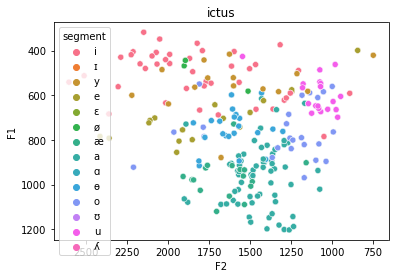
\includegraphics[width=0.70\columnwidth]{figures/ictus}
%\caption{{vowel chart for all vowels in ictus position
%{\label{198139}}%
%}}
%
%\end{figure}
%\begin{figure}
%
%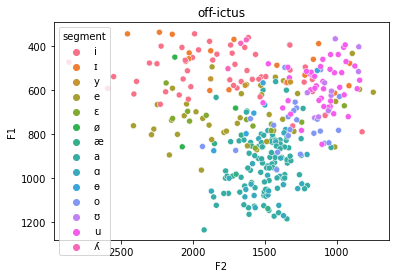
\includegraphics[width=0.70\columnwidth]{figures/off-ictus}
%\caption{{vowel chart for all vowels in off-ictus position
%{\label{146554}}%
%}}
%\end{figure}
%%
%%
%
%\begin{figure}[H]
%\begin{center}
%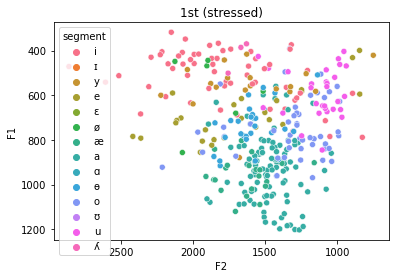
\includegraphics[width=0.70\columnwidth]{figures/first}
%\caption{{vowel space for stressed syllables
%{\label{216251}}%
%}}
%\end{center}
%\end{figure}
%
%\begin{figure}[H]
%\begin{center}
%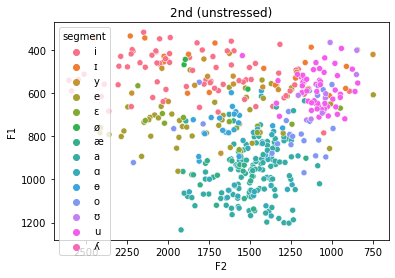
\includegraphics[width=0.70\columnwidth]{figures/second}
%\caption{{vowel space for unstressed syllables
%{\label{971548}}%
%}}
%\end{center}
%\end{figure}



%Introducing the graphs:
%\begin{figure}[H]
%\begin{center}
%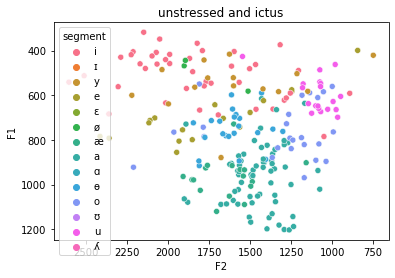
\includegraphics[width=0.70\columnwidth]{figures/unstressed-ictus}
%\caption{{Vowel Space of word-weak syllables in song-strong positions (conflicting
%prominence)
%{\label{632826}}%
%}}
%\end{center}
%\end{figure}\selectlanguage{english}
%\begin{figure}[H]
%\begin{center}
%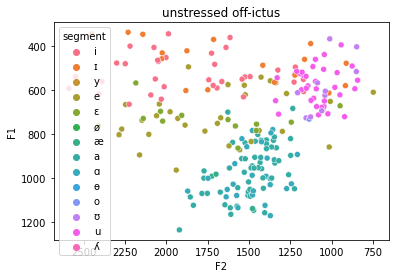
\includegraphics[width=0.70\columnwidth]{figures/unstressedoff-ictus}
%\caption{{Vowel Space of word-weak syllables in song-weak positions (concordant
%prominence)
%{\label{853436}}%
%}}
%\end{center}
%\end{figure}
%
%statistical analysis of word-weak combinations
%
%introducing the next graphs: song-strong conflicts\selectlanguage{english}
%\begin{figure}[H]
%\begin{center}
%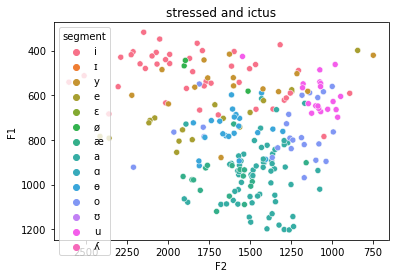
\includegraphics[width=0.70\columnwidth]{figures/stressed-ictus}
%\caption{{Vowel Space of word-strong syllables in song-weak positions (conflicting
%prominence)
%{\label{888534}}%
%}}
%\end{center}
%\end{figure}
%
%we'll say more things here
%\begin{figure}[H]
%\begin{center}
%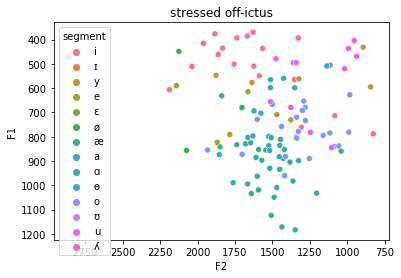
\includegraphics[width=0.70\columnwidth]{figures/stressedoff-ictus}
%\caption{{vowel space of word-strong syllables in song-weak positions (conflicting
%prominence)%
%}}
%\end{center}
%\end{figure}
%
%
%saying things \\
\pagebreak
\section*{Discussion}

The results confirm the findings of Ross \& Lehiste's studies on timing in Estonian folk songs, while illuminating potential signatures of prominence contrast preservation when duration is lost to the song. Vowel duration usually increases with syllable prominence at the word level but, in sung verse, decreases as syllable weight or prominence increases. In order to confirm foot and note isochrony, the next logical step is to measure whole syllables and words and their relative proportions. Measuring onset consonant duration will potentially illuminate the vowel shortening in stressed syllables. 

%The EFA houses an extensive database of 20th century Estonian songs and stories in a variety of physical and digital formats. \\
% Stress in Estonian is acoustically most often realized by onset consonant lengthening (Gordon, 1997; Hint, 1973). Gordon 1997 also found evidence for acoustic correlates of prosodic domains by measuring peak nasal flow, nasal amplitude, and duration in initial positions of four prosodic domains. The syllable, word, phrase, and utterance, were each also cross-classified for stressed and unstressed positions. \\
% 
% 
%%functional load hypothesis \cite{berinsteinWPPNo471979} \\
%but another cross-linguistic study specifically analyzed the acoustic correlates of stress in languages that have a duration contrast, and found no support for the functional load hypothesis (Lunden et al., 2017). Thus this study has another potential theoretical bearing to weigh in on. 

%.The lowered amplitude of initial nasal segments (also found by (Fougeron 1996)), Gordon argues, is to maximize consonantness compared to the sonorance of the following vowel. Nasal data provided evidence for progressively larger domains of prosodic constituency: syllable, word, and phrase. 
%
%Previous research has shown lengthening of domain-final segments (Oller 1973, Beckman et al 1992, Wightman et al 1992), wherein the higher the prosodic level, the greater the lengthening effect in general. Will this remain the case at different levels of the prosodic domain of the song?


%More recent work has found that proportional duration increases \cite{Lunden} between adjacent syllables is a more robust metric than simple duration ratio. 
%\subsection{Syllable index within phrase compared to beats detected}
%\begin{itemize}
%\item rate of beats/syllables in each song
%\item occurence of beats in odd (ictus) syllables
%\item beats detected outside of ictus
%\item overall robustness of the beat detection
%\end{itemize}
%\subsection{Duration Ratios:} 
%\subsubsection*{metrical analysis of text database of {\it regilaul}}
% a text database of {\it regilaul} songs: \url{https://www.folklore.ee/regilaul/andmebaas/?ln=en}. With this, I will analyze the frequency of stress and ictus conflicts in the larger pool of songs.  For example, are there more occurrences of syllables strong at the word level ending up in weak metrical positions, or more weak word-level syllables in strong metrical positions? How often do overlong (Q3, heaviest possible) syllables end up in metrically weak positions, if at all? \\
%In addition, looking forward to the future when I expand this corpus, I may strategize using the database to find songs that have several of the song and word stress conflicts that I am looking for. As these are folk songs, there will be multiple recordings of a given song, sometimes to different melodies or in different dialects. There would, of course, need to be a balance of songs where there are few or no conflicts to compare measurements to, but analyzing the database could also help to locate those. \\
%At the very least, this database can provide some useful data, such as lexical frequency within the broader set of regilaul songs to provide a gradient picture of the present corpus in the context of {\it regilaul} songs on the whole. 

%\subsection{Growing the Corpus} 
%Available on the archive are eight more songs from the same region and time period, which would bring the total songs to 17 {\it regilaul} songs and seven singers. Once these annotations are aligned and verified, the audio corpus will total thirty-two minutes and twelve seconds of recorded audio. 

\section*{Conclusion}

Vowel Duration: \\
We failed to reject the null hypothesis for vowel duration: while the song level does dominate the temporal domain, there is an inverse relationship to vowel duration and word-level duration contrasts for Q1, Q3, and stressed syllables. So while the song always wins, there is clearly something else going on. It is possible that it is as simple as note-syllable isochrony, and the vowel decrease is simply an accommodation to give the ictus level the appropriate duration syllable. 

Vowel Space: \\

After confirming that song position is the dominant hierarchy for temporal constraints, we continue on to see how vowel space plays out in different levels of prosodic prominence. We are able to reject the null hypothesis with data to support a clear relationship between prominence and vowel space, this time at both prosodic levels (song and word.) This suggests that for the song, ``preserve contrast" ranks lower than the temporal constraints, but that so long as the strong positions in the song are satisfied, prominence can be indicated by vowel space at multiple levels of the prosodic hierarchy.  



\bibliographystyle{apalike}
\bibliography{QP.bib}
\end{document}

%\section*{References}\sloppy
%\phantomsection
%\label{csl:1}\textit{{Anthology of {{Estonian Traditional Music}}}}. \url{https://www.folklore.ee/pubte/eraamat/rahvamuusika/en/index.}
%
%\phantomsection
%\label{csl:2}\textit{{Praat: Doing {{Phonetics}} by {{Computer}}}}. \url{https://www.fon.hum.uva.nl/praat/.}

%\appendix
%\section{vowel data}
%
%\begin{tabular}{lrlrllllrrlrrrll}
%\toprule
%& Index &             word &  word\_dur &    syll & quantity & stress & segment &  seg\_duration &  seg\_midpoint &  ictus &           f1 &           f2 &          euc & fileid & performer \\
%\midrule
%1    &           1 &            pandi &  0.456740 &     pan &        2 &      1 &       a &      0.177026 &      6.947528 &  ictus &   603.056801 &  1303.781807 &   700.725006 &     65 &        LK \\
%4    &           4 &            pandi &  0.456740 &      di &        1 &      0 &       i &      0.129039 &      7.202174 &    off &  1074.849998 &  2167.095173 &  1092.245175 &     65 &        LK \\
%6    &           6 &          mind(e) &  0.292967 &    mind &        2 &      1 &       i &      0.085210 &      7.364037 &    off &   731.376613 &  1651.342030 &   919.965417 &     65 &        LK \\
%9    &           9 &          mind(e) &  0.292967 &     (e) &        2 &      0 &       e &      0.067737 &      7.527525 &    off &   852.719874 &  1444.954754 &   592.234880 &     65 &        LK \\
%11   &          11 &             paju &  0.881775 &      pa &        1 &      1 &       a &      0.386617 &      7.887546 &  ictus &   794.798321 &   850.845027 &    56.046706 &     65 &        LK \\
%15   &          15 &        raiumaie, &  1.569131 &     rai &        2 &      1 &       a &      0.170306 &      8.642248 &  ictus &   607.479426 &  1794.748145 &  1187.268720 &     65 &        LK \\
%16   &          16 &        raiumaie, &  1.569131 &     rai &        2 &      1 &       i &      0.121106 &      8.787954 &  ictus &   639.850023 &  1179.760877 &   539.910854 &     65 &        LK \\
%25   &          25 &            saare &  0.770835 &      re &        1 &      0 &       e &      0.219092 &     14.344008 &    off &   942.303095 &  1513.288115 &   570.985020 &     65 &        LK \\
%\bottomrule
%\toprule
%& Index &             word &  word\_dur &    syll & quantity & stress & segment &  seg\_duration &  seg\_midpoint &  ictus &           f1 &           f2 &          euc & fileid & performer \\
%\midrule
%29   &          29 &            juuri &  0.850004 &      ri &        1 &      0 &       i &      0.251226 &     15.177945 &    off &   495.140100 &   929.235290 &   434.095189 &     65 &        LK \\
%31   &          31 &       juksimaie, &  1.576455 &     juk &        2 &      0 &       u &      0.211732 &     15.477062 &  ictus &   593.905746 &  1099.944478 &   506.038732 &     65 &        LK \\
%34   &          34 &       juksimaie, &  1.576455 &      si &        1 &      0 &       i &      0.269766 &     15.932366 &  ictus &   609.070147 &  1377.042100 &   767.971952 &     65 &        LK \\
%36   &          36 &       juksimaie, &  1.576455 &     mai &        2 &      1 &       a &      0.199649 &     16.278424 &  ictus &  1219.144093 &  2219.320728 &  1000.176635 &     65 &        LK \\
%37   &          37 &       juksimaie, &  1.576455 &     mai &        2 &      1 &       i &      0.066408 &     16.411452 &  ictus &   567.793964 &  1517.588974 &   949.795010 &     65 &        LK \\
%40   &          40 &            tamme &  0.800402 &     tam &        2 &      1 &       a &      0.262818 &     20.290343 &  ictus &   867.436511 &  1405.601686 &   538.165175 &     65 &        LK \\
%43   &          43 &            tamme &  0.800402 &      me &        1 &      0 &       e &      0.225586 &     20.725088 &    off &   871.247913 &  1444.924978 &   573.677065 &     65 &        LK \\
%49   &          49 &       tampimaie. &  1.566424 &     tam &        2 &      0 &       a &      0.168642 &     21.870669 &  ictus &   681.121800 &  1808.088733 &  1126.966932 &     65 &        LK \\
%52   &          52 &       tampimaie. &  1.566424 &      pi &        1 &      0 &       i &      0.282127 &     22.376392 &    off &   967.673507 &  1494.563480 &   526.889973 &     65 &        LK \\
%54   &          54 &       tampimaie. &  1.566424 &     mai &        2 &      1 &       a &      0.180266 &     22.715309 &  ictus &   949.413512 &  1535.988601 &   586.575090 &     65 &        LK \\
%55   &          55 &       tampimaie. &  1.566424 &     mai &        2 &      1 &       i &      0.088005 &     22.849444 &  ictus &   562.462719 &  1850.910966 &  1288.448247 &     65 &        LK \\
%58   &          58 &         Leidsine &  0.846330 &    leid &        2 &      1 &       e &      0.190682 &     27.801953 &  ictus &  1172.794519 &  2308.019967 &  1135.225448 &     65 &        LK \\
%\bottomrule
%\toprule
%& Index &             word &  word\_dur &    syll & quantity & stress & segment &  seg\_duration &  seg\_midpoint &  ictus &           f1 &           f2 &          euc & fileid & performer \\
%\midrule
%59   &          59 &         Leidsine &  0.846330 &    leid &        2 &      1 &       i &      0.165144 &     27.979866 &  ictus &   936.416877 &  2142.988692 &  1206.571814 &     65 &        LK \\
%62   &          62 &         Leidsine &  0.846330 &      si &        1 &      0 &       i &      0.047671 &     28.253120 &    off &   568.151391 &  2315.836378 &  1747.684987 &     65 &        LK \\
%64   &          64 &         Leidsine &  0.846330 &      ne &        1 &      0 &       e &      0.108035 &     28.375238 &    off &   665.673846 &  1598.382843 &   932.708997 &     65 &        LK \\
%66   &          66 &               ma &  0.506563 &      ma &        3 &      1 &       a &      0.414011 &     28.728813 &  ictus &  1053.220537 &  2443.320171 &  1390.099634 &     65 &        LK \\
%68   &          68 &             siis &  0.320944 &    siis &        3 &      1 &       i &      0.115491 &     29.069516 &    off &   914.374090 &  1337.084690 &   422.710601 &     65 &        LK \\
%71   &          71 &        kogemata, &  1.787757 &      ko &        1 &      1 &       o &      0.372798 &     29.568103 &  ictus &   408.161971 &  2056.293211 &  1648.131240 &     65 &        LK \\
%75   &          75 &        kogemata, &  1.787757 &      ma &        2 &      0 &       a &      0.186399 &     30.329769 &  ictus &   704.669172 &  1275.958334 &   571.289162 &     65 &        LK \\
%77   &          77 &        kogemata, &  1.787757 &     ta, &        2 &      0 &       a &      0.400871 &     30.844084 &    off &   973.486795 &  1258.895949 &   285.409154 &     65 &        LK \\
%79   &          79 &              kus &  0.504272 &     kus &        3 &      1 &       u &      0.263281 &     34.715544 &  ictus &   876.381449 &  2356.215364 &  1479.833915 &     65 &        LK \\
%81   &          81 &              aga &  0.280212 &       a &        1 &      1 &       a &      0.103108 &     35.079497 &    off &   626.628378 &  2150.116222 &  1523.487844 &     65 &        LK \\
%85   &          85 &             salk &  0.546964 &    salk &        3 &      1 &       a &      0.218522 &     35.495419 &  ictus &   577.666135 &  2027.925656 &  1450.259520 &     65 &        LK \\
%88   &          88 &              oli &  0.336032 &       o &        1 &      1 &       o &      0.128193 &     35.919215 &  ictus &   792.680336 &  1782.100047 &   989.419711 &     65 &        LK \\
%92   &          92 &       sarapuida, &  1.654125 &      sa &        1 &      0 &       a &      0.379503 &     36.488923 &  ictus &   831.314916 &  1484.301287 &   652.986371 &     65 &        LK \\
%96   &          96 &       sarapuida, &  1.654125 &     pui &        2 &      1 &       u &      0.184549 &     37.278897 &  ictus &   738.795271 &  1711.982499 &   973.187229 &     65 &        LK \\
%97   &          97 &       sarapuida, &  1.654125 &     pui &        2 &      1 &       i &      0.166604 &     37.454473 &  ictus &   847.558657 &  1426.912543 &   579.353885 &     65 &        LK \\
%99   &          99 &       sarapuida, &  1.654125 &     da, &        2 &      0 &       a &      0.242105 &     37.724224 &    off &   676.553409 &  1163.692724 &   487.139315 &     65 &        LK \\
%101  &         101 &            teine &  0.819799 &     tei &        2 &      1 &       e &      0.249376 &     42.353548 &  ictus &   945.369729 &  1470.322559 &   524.952830 &     65 &        LK \\
%102  &         102 &            teine &  0.819799 &     tei &        2 &      1 &       i &      0.172249 &     42.564361 &  ictus &   867.860811 &  1923.174803 &  1055.313991 &     65 &        LK \\
%104  &         104 &            teine &  0.819799 &      ne &        1 &      0 &       e &      0.239816 &     42.846476 &    off &   550.773852 &  1837.178751 &  1286.404899 &     65 &        LK \\
%106  &         106 &             salk &  0.543072 &    salk &        3 &      1 &       a &      0.203542 &     43.147736 &  ictus &   484.985512 &  1062.590544 &   577.605032 &     65 &        LK \\
%109  &         109 &              oli &  0.290331 &       o &        1 &      1 &       o &      0.110688 &     43.564801 &  ictus &   605.174299 &  2005.970684 &  1400.796385 &     65 &        LK \\
%116  &         116 &      türnapuida, &  1.827076 &      na &        2 &      0 &       a &      0.250439 &     44.462075 &  ictus &   665.067678 &  1545.082186 &   880.014508 &     65 &        LK \\
%118  &         118 &      türnapuida, &  1.827076 &     pui &        2 &      1 &       u &      0.150628 &     44.843305 &  ictus &   555.848896 &  1658.742905 &  1102.894009 &     65 &        LK \\
%119  &         119 &      türnapuida, &  1.827076 &     pui &        2 &      1 &       i &      0.187000 &     45.012119 &  ictus &   965.804056 &  1435.653848 &   469.849792 &     65 &        LK \\
%121  &         121 &      türnapuida, &  1.827076 &     da, &        2 &      0 &       a &      0.443587 &     45.405070 &    off &   567.284920 &  1145.634132 &   578.349212 &     65 &        LK \\
%123  &         123 &           kolmas &  0.872814 &     kol &        2 &      1 &       o &      0.248276 &     49.353748 &  ictus &   982.247255 &  1948.946556 &   966.699301 &     65 &        LK \\
%126  &         126 &           kolmas &  0.872814 &     mas &        2 &      0 &       a &      0.196874 &     49.806823 &    off &   594.887414 &  1037.968440 &   443.081026 &     65 &        LK \\
%129  &         129 &             salk &  0.517537 &    salk &        3 &      1 &       a &      0.241793 &     50.189175 &  ictus &   520.044473 &  1197.177914 &   677.133442 &     65 &        LK \\
%132  &         132 &              oli &  0.323880 &       o &        1 &      1 &       o &      0.113363 &     50.588171 &    off &   951.648529 &  1777.618110 &   825.969581 &     65 &        LK \\
%136  &         136 &      kohlapuida, &  1.616739 &     koh &        2 &      0 &       o &      0.279816 &     51.099187 &  ictus &   755.172487 &  1160.045987 &   404.873500 &     65 &        LK \\
%139  &         139 &      kohlapuida, &  1.616739 &      la &        2 &      0 &       a &      0.218393 &     51.582610 &    off &   703.407720 &  1256.477090 &   553.069370 &     65 &        LK \\
%141  &         141 &      kohlapuida, &  1.616739 &     pui &        2 &      1 &       u &      0.245693 &     51.964799 &  ictus &   520.081829 &  1404.904199 &   884.822371 &     65 &        LK \\
%142  &         142 &      kohlapuida, &  1.616739 &     pui &        2 &      1 &       i &      0.166070 &     52.170680 &  ictus &   861.016763 &  1416.021473 &   555.004710 &     65 &        LK \\
%144  &         144 &      kohlapuida, &  1.616739 &     da, &        2 &      0 &       a &      0.172895 &     52.385661 &    off &   771.013138 &  1008.549936 &   237.536799 &     65 &        LK \\
%146  &         146 &           neljas &  1.009473 &     nel &        2 &      1 &       e &      0.287265 &     57.358765 &  ictus &  1197.168693 &  2141.033928 &   943.865235 &     65 &        LK \\
%149  &         149 &           neljas &  1.009473 &     jas &        2 &      0 &       a &      0.228961 &     57.875510 &    off &   672.717937 &  1988.246307 &  1315.528370 &     65 &        LK \\
%154  &         154 &            noori &  0.884473 &      ri &        1 &      0 &       i &      0.223008 &     58.827216 &    off &  1053.796896 &  1452.524986 &   398.728090 &     65 &        LK \\
%156  &         156 &       neidusida, &  1.820135 &     nei &        2 &      1 &       e &      0.185210 &     59.152279 &  ictus &   775.172423 &  1439.125289 &   663.952866 &     65 &        LK \\
%157  &         157 &       neidusida, &  1.820135 &     nei &        2 &      1 &       i &      0.143632 &     59.316700 &  ictus &   646.473833 &  1524.014230 &   877.540398 &     65 &        LK \\
%159  &         159 &       neidusida, &  1.820135 &      du &        1 &      0 &       u &      0.366012 &     59.650898 &    off &   639.544828 &  1424.797404 &   785.252575 &     65 &        LK \\
%161  &         161 &       neidusida, &  1.820135 &      si &        1 &      0 &       i &      0.336402 &     60.085889 &  ictus &   553.621937 &  1109.595091 &   555.973154 &     65 &        LK \\
%163  &         163 &       neidusida, &  1.820135 &     da, &        2 &      0 &       a &      0.410270 &     60.553720 &    off &   523.296667 &  2675.973493 &  2152.676826 &     65 &        LK \\
%165  &         165 &       punapõs ki &  1.723722 &      pu &        1 &      1 &       u &      0.419013 &     64.587020 &  ictus &  1144.960285 &  2258.740399 &  1113.780114 &     65 &        LK \\
%176  &         176 &       piigakesi. &  1.845679 &      ga &        2 &      0 &       a &      0.284715 &     66.737920 &  ictus &   434.472103 &  1255.131584 &   820.659481 &     65 &        LK \\
%178  &         178 &       piigakesi. &  1.845679 &      ke &        1 &      0 &       e &      0.350419 &     67.217555 &  ictus &   849.175124 &  1555.399005 &   706.223881 &     65 &        LK \\
%180  &         180 &       piigakesi. &  1.845679 &     si. &        2 &      0 &       i &      0.330730 &     67.683272 &    off &   557.631391 &  1336.701623 &   779.070231 &     65 &        LK \\
%184  &         184 &             neil &  0.393891 &    neil &        3 &      1 &       e &      0.132287 &     72.481424 &    off &   416.163656 &  1716.677615 &  1300.513959 &     65 &        LK \\
%185  &         185 &             neil &  0.393891 &    neil &        3 &      1 &       i &      0.113344 &     72.604239 &    off &   471.237457 &  1983.635140 &  1512.397684 &     65 &        LK \\
%189  &         189 &            ööles &  0.892748 &     les &        2 &      0 &       e &      0.242808 &     73.406274 &    off &   498.468469 &  1506.749397 &  1008.280928 &     65 &        LK \\
%192  &         192 &      virvekirja, &  1.858469 &     vir &        2 &      1 &       i &      0.223044 &     73.903795 &  ictus &   938.982156 &  1663.175662 &   724.193506 &     65 &        LK \\
%195  &         195 &      virvekirja, &  1.858469 &      ve &        1 &      0 &       e &      0.273865 &     74.383764 &    off &   621.651584 &  1268.414515 &   646.762932 &     65 &        LK \\
%197  &         197 &      virvekirja, &  1.858469 &     kir &        2 &      1 &       i &      0.233053 &     74.752979 &  ictus &   569.024102 &  1573.040181 &  1004.016078 &     65 &        LK \\
%200  &         200 &      virvekirja, &  1.858469 &     ja, &        2 &      0 &       a &      0.363467 &     75.329212 &    off &   527.059622 &  1584.852237 &  1057.792615 &     65 &        LK \\
%202  &         202 &            sukad &  0.929223 &      su &        2 &      1 &       u &      0.272400 &     79.373665 &  ictus &   978.912689 &  2181.856913 &  1202.944224 &     65 &        LK \\
%204  &         204 &            sukad &  0.929223 &     kad &        2 &      0 &       a &      0.205931 &     79.828499 &    off &   539.061419 &  1268.707004 &   729.645585 &     65 &        LK \\
%207  &         207 &            jalas &  0.843003 &      ja &        1 &      1 &       a &      0.346229 &     80.363895 &  ictus &   941.087899 &  1482.908322 &   541.820424 &     65 &        LK \\
%214  &         214 &      saarekirja. &  1.903127 &      re &        1 &      0 &       e &      0.306513 &     81.659703 &  ictus &   916.108796 &  1298.080154 &   381.971357 &     65 &        LK \\
%216  &         216 &      saarekirja. &  1.903127 &     kir &        2 &      1 &       i &      0.238683 &     82.049689 &  ictus &   598.976764 &  1878.631215 &  1279.654451 &     65 &        LK \\
%219  &         219 &      saarekirja. &  1.903127 &     ja. &        2 &      0 &       a &      0.381306 &     82.614691 &    off &   541.695026 &  1803.498187 &  1261.803160 &     65 &        LK \\
%220  &         220 &               Ei &  0.580891 &      ei &        3 &      1 &       e &      0.239473 &     86.945032 &  ictus &   828.275768 &  2099.677150 &  1271.401382 &     65 &        LK \\
%222  &         222 &             olnd &  0.454681 &    olnd &        3 &      1 &       o &      0.201667 &     87.451928 &    off &   510.440013 &  1321.558180 &   811.118166 &     65 &        LK \\
%227  &         227 &          julgust &  0.853375 &     jul &        2 &      1 &       u &      0.192606 &     87.992288 &  ictus &   715.106874 &  1191.176407 &   476.069534 &     65 &        LK \\
%230  &         230 &          julgust &  0.853375 &    gust &        2 &      0 &       u &      0.181597 &     88.391662 &    off &   491.030890 &  1336.437823 &   845.406933 &     65 &        LK \\
%236  &         236 &            juure &  0.837714 &      re &        1 &      0 &       e &      0.327787 &     89.332971 &  ictus &   610.036521 &   979.472257 &   369.435736 &     65 &        LK \\
%238  &         238 &           minna, &  0.753516 &     min &        2 &      1 &       i &      0.187944 &     89.706788 &  ictus &   542.499425 &  1839.671911 &  1297.172486 &     65 &        LK \\
%241  &         241 &           minna, &  0.753516 &     na, &        2 &      0 &       a &      0.143127 &     90.103639 &  ictus &   538.171963 &   931.002427 &   392.830464 &     65 &        LK \\
%252  &         252 &            sülle &  0.838747 &      le &        1 &      0 &       e &      0.308579 &     95.744141 &  ictus &   564.813217 &  1809.842226 &  1245.029009 &     65 &        LK \\
%254  &         254 &        rabadaie. &  1.616668 &      ra &        1 &      0 &       a &      0.333783 &     96.176488 &  ictus &   725.244483 &  1523.765777 &   798.521294 &     65 &        LK \\
%258  &         258 &        rabadaie. &  1.616668 &     dai &        2 &      1 &       a &      0.201661 &     96.979654 &  ictus &   868.098454 &  1223.003465 &   354.905011 &     65 &        LK \\
%259  &         259 &        rabadaie. &  1.616668 &     dai &        2 &      1 &       i &      0.111261 &     97.136115 &  ictus &   813.632222 &  1452.202956 &   638.570734 &     65 &        LK \\
%262  &           1 &            Kelle &  0.548370 &     kel &        2 &      1 &       e &      0.224554 &      0.116470 &  ictus &  1110.553772 &  2154.184673 &  1043.630900 &     77 &        LO \\
%265  &           4 &            Kelle &  0.548370 &      le &        1 &      0 &       e &      0.188403 &      0.454169 &    off &   699.571764 &  1442.320280 &   742.748516 &     77 &        LO \\
%266  &           5 &             olid &  0.241858 &       o &        1 &      1 &       o &      0.079548 &      8.579695 &    off &   565.393103 &  1360.381869 &   794.988766 &     77 &        LO \\
%270  &           9 &             olid &  0.263388 &       o &        1 &      1 &       o &      0.090110 &     13.836824 &  ictus &   600.776086 &  1829.111356 &  1228.335269 &     77 &        LO \\
%274  &          13 &              oli &  0.241781 &       o &        1 &      1 &       o &      0.091616 &     18.811614 &    off &   344.256845 &  1708.222583 &  1363.965738 &     77 &        LO \\
%280  &          19 &            neede &  0.333389 &      de &        1 &      0 &       e &      0.138341 &     21.950581 &  ictus &   438.048551 &   877.384334 &   439.335783 &     77 &        LO \\
%283  &          22 &           tõusis &  0.381856 &     tõu &        2 &      1 &       u &      0.049156 &     29.103598 &    off &   706.602277 &  1956.508763 &  1249.906487 &     77 &        LO \\
%285  &          24 &           tõusis &  0.381856 &     sis &        2 &      0 &       i &      0.080565 &     29.217459 &    off &   617.763323 &  1444.108386 &   826.345062 &     77 &        LO \\
%287  &          26 &              oli &  0.189509 &       o &        1 &      1 &       o &      0.086880 &     39.208823 &    off &   528.944769 &  1335.684405 &   806.739636 &     77 &        LO \\
%\bottomrule
%\toprule
%& Index &             word &  word\_dur &    syll & quantity & stress & segment &  seg\_duration &  seg\_midpoint &  ictus &           f1 &           f2 &          euc & fileid & performer \\
%\midrule
%290  &          29 &            akkas &  0.277614 &      ak &        3 &      1 &       a &      0.086659 &     47.267502 &    off &   941.484750 &  1859.900331 &   918.415581 &     77 &        LO \\
%295  &          34 &         korjama. &  0.941133 &     kor &        2 &      1 &       o &      0.179652 &     50.715728 &  ictus &   748.536279 &  1101.027221 &   352.490942 &     77 &        LO \\
%298  &          37 &         korjama. &  0.941133 &      ja &        1 &      0 &       a &      0.149135 &     51.093565 &    off &   775.115910 &  1225.596926 &   450.481016 &     77 &        LO \\
%300  &          39 &         korjama. &  0.941133 &     ma. &        2 &      0 &       a &      0.152562 &     51.363946 &  ictus &   520.557155 &  1783.342514 &  1262.785359 &     77 &        LO \\
%301  &          40 &           akkase &  0.544724 &      ak &        3 &      1 &       a &      0.217503 &     54.508593 &  ictus &   775.524440 &  1467.833189 &   692.308749 &     77 &        LO \\
%309  &          48 &            neede &  0.253786 &      de &        1 &      0 &       e &      0.088892 &     69.694035 &    off &  1018.803389 &  2019.146070 &  1000.342681 &     77 &        LO \\
%311  &          50 &             pani &  0.257474 &      pa &        1 &      1 &       a &      0.113842 &     74.318024 &    off &  1120.920587 &  1967.975410 &   847.054823 &     77 &        LO \\
%315  &          54 &        taevudes, &  0.901312 &     tae &        2 &      1 &       a &      0.192910 &     77.807736 &    off &   372.649916 &   817.903765 &   445.253849 &     77 &        LO \\
%316  &          55 &        taevudes, &  0.901312 &     tae &        2 &      1 &       e &      0.139361 &     77.973871 &  ictus &   383.738623 &  1460.733601 &  1076.994977 &     77 &        LO \\
%318  &          57 &        taevudes, &  0.901312 &      vu &        1 &      0 &       u &      0.137478 &     78.171291 &  ictus &   764.949395 &  1781.883282 &  1016.933887 &     77 &        LO \\
%320  &          59 &        taevudes, &  0.901312 &    des, &        3 &      1 &       e &      0.132039 &     78.389291 &  ictus &   764.710976 &  1504.974307 &   740.263331 &     77 &        LO \\
%323  &           1 &            Laske &  0.700087 &     las &        2 &      1 &       a &      0.221538 &      0.179564 &  ictus &  1125.029770 &  2441.781428 &  1316.751658 &     18 &        MH \\
%326  &           4 &            Laske &  0.700087 &      ke &        1 &      0 &       e &      0.232149 &      0.584012 &  ictus &   895.423885 &  1680.387334 &   784.963450 &     18 &        MH \\
%328  &           6 &            sissi &  0.700410 &     sis &        2 &      1 &       i &      0.182000 &      0.895047 &  ictus &   646.991170 &  1970.239031 &  1323.247861 &     18 &        MH \\
%331  &           9 &            sissi &  0.700410 &      si &        1 &      0 &       i &      0.215953 &      1.292520 &    off &   408.900806 &  1927.619804 &  1518.718998 &     18 &        MH \\
%333  &          11 &      kadrisandi, &  1.452924 &     kad &        2 &      1 &       a &      0.261981 &      1.631550 &  ictus &   487.272400 &  2095.257038 &  1607.984639 &     18 &        MH \\
%336  &          14 &      kadrisandi, &  1.452924 &      ri &        1 &      0 &       i &      0.173960 &      2.010561 &    off &   915.827585 &  1624.240810 &   708.413226 &     18 &        MH \\
%338  &          16 &      kadrisandi, &  1.452924 &     san &        2 &      1 &       a &      0.212000 &      2.318541 &  ictus &   555.975211 &  2245.446401 &  1689.471190 &     18 &        MH \\
%341  &          19 &      kadrisandi, &  1.452924 &     di, &        2 &      0 &       i &      0.217572 &      2.744634 &    off &   987.703400 &  1651.780514 &   664.077114 &     18 &        MH \\
%343  &          21 &            Laske &  0.665724 &     las &        2 &      1 &       a &      0.166557 &      5.768753 &  ictus &   869.919401 &  2374.105112 &  1504.185711 &     18 &        MH \\
%346  &          24 &            Laske &  0.665724 &      ke &        1 &      0 &       e &      0.176658 &      6.128450 &    off &   879.889375 &  1576.797396 &   696.908022 &     18 &        MH \\
%348  &          26 &            sissi &  0.666013 &     sis &        2 &      1 &       i &      0.178000 &      6.413280 &  ictus &   594.097939 &  2338.073084 &  1743.975145 &     18 &        MH \\
%351  &          29 &            sissi &  0.666013 &      si &        1 &      0 &       i &      0.177256 &      6.794164 &  ictus &   573.828713 &  1903.269133 &  1329.440420 &     18 &        MH \\
%353  &          31 &      kadrisandi, &  1.335653 &     kad &        2 &      1 &       a &      0.248754 &      7.105154 &  ictus &   506.428408 &  1807.366099 &  1300.937690 &     18 &        MH \\
%356  &          34 &      kadrisandi, &  1.335653 &      ri &        1 &      0 &       i &      0.175548 &      7.443978 &  ictus &  1060.101356 &  1622.578059 &   562.476703 &     18 &        MH \\
%358  &          36 &      kadrisandi, &  1.335653 &     san &        2 &      1 &       a &      0.187000 &      7.713030 &  ictus &   615.238571 &  2124.478740 &  1509.240169 &     18 &        MH \\
%361  &          39 &      kadrisandi, &  1.335653 &     di, &        2 &      0 &       i &      0.176915 &      8.129988 &    off &   905.970476 &  1665.661237 &   759.690761 &     18 &        MH \\
%363  &          41 &           kadril &  0.722073 &     kad &        2 &      1 &       a &      0.238375 &     10.904961 &  ictus &   914.385671 &  2211.975322 &  1297.589651 &     18 &        MH \\
%366  &          44 &           kadril &  0.722073 &     ril &        2 &      0 &       i &      0.137863 &     11.275080 &    off &  1187.177770 &  1401.988153 &   214.810382 &     18 &        MH \\
%376  &          54 &       külmeteve, &  1.347786 &      me &        2 &      0 &       e &      0.149118 &     12.551383 &    off &   521.867049 &  2026.077997 &  1504.210948 &     18 &        MH \\
%378  &          56 &       külmeteve, &  1.347786 &      te &        1 &      0 &       e &      0.317215 &     12.936380 &  ictus &   835.447166 &  1536.479817 &   701.032651 &     18 &        MH \\
%380  &          58 &       külmeteve, &  1.347786 &     ve, &        2 &      0 &       e &      0.207927 &     13.275802 &    off &   561.223316 &  1747.259347 &  1186.036032 &     18 &        MH \\
%382  &          60 &           kadril &  0.725727 &     kad &        2 &      1 &       a &      0.240987 &     16.165461 &  ictus &   667.046434 &  2158.647567 &  1491.601133 &     18 &        MH \\
%385  &          63 &           kadril &  0.725727 &     ril &        2 &      0 &       i &      0.114419 &     16.499140 &    off &  1134.339837 &  1244.181324 &   109.841487 &     18 &        MH \\
%388  &          66 &            varba &  0.635000 &     var &        2 &      1 &       a &      0.153886 &     16.777314 &  ictus &   612.376360 &  1828.205161 &  1215.828801 &     18 &        MH \\
%391  &          69 &            varba &  0.635000 &      ba &        1 &      0 &       a &      0.230308 &     17.170763 &  ictus &   977.373724 &  1506.843211 &   529.469487 &     18 &        MH \\
%393  &          71 &        valutave! &  1.192302 &      va &        1 &      1 &       a &      0.246613 &     17.466962 &  ictus &  1104.298647 &  1456.355060 &   352.056413 &     18 &        MH \\
%397  &          75 &        valutave! &  1.192302 &      ta &        1 &      0 &       a &      0.222938 &     18.060806 &  ictus &   717.926385 &  1109.852597 &   391.926212 &     18 &        MH \\
%399  &          77 &        valutave! &  1.192302 &     ve! &        2 &      0 &       e &      0.229001 &     18.363718 &    off &   885.102350 &  1683.137468 &   798.035118 &     18 &        MH \\
%401  &          79 &            Kadri &  0.417147 &     kad &        2 &      1 &       a &      0.136252 &     21.157477 &  ictus &   867.395664 &  2271.157447 &  1403.761783 &     18 &        MH \\
%404  &          82 &            Kadri &  0.417147 &      ri &        1 &      0 &       i &      0.053933 &     21.380306 &    off &   728.269642 &  1824.428184 &  1096.158542 &     18 &        MH \\
%405  &          83 &               om &  0.257651 &      om &        3 &      1 &       o &      0.181669 &     21.498107 &    off &  1008.627270 &  1523.729941 &   515.102671 &     18 &        MH \\
%408  &          86 &            tullu &  0.598432 &     tul &        2 &      1 &       u &      0.205348 &     21.844899 &  ictus &   691.683512 &  1496.844247 &   805.160735 &     18 &        MH \\
%411  &          89 &            tullu &  0.598432 &      lu &        1 &      0 &       u &      0.143836 &     22.191438 &    off &   673.196901 &  1080.966859 &   407.769958 &     18 &        MH \\
%413  &          91 &            kauge &  0.694534 &     kau &        2 &      1 &       a &      0.244117 &     22.472785 &  ictus &   629.653437 &  1479.338462 &   849.685025 &     18 &        MH \\
%416  &          94 &            kauge &  0.694534 &      ge &        1 &      0 &       e &      0.198215 &     22.856696 &    off &   926.911664 &  1422.632238 &   495.720574 &     18 &        MH \\
%423  &         101 &           ümmert &  0.758560 &    mert &        2 &      0 &       e &      0.157399 &     26.747851 &    off &   505.746178 &  1414.781439 &   909.035261 &     18 &        MH \\
%426  &         104 &            ilma, &  0.654445 &      il &        2 &      1 &       i &      0.210045 &     27.055780 &  ictus &   906.229386 &  2058.170929 &  1151.941543 &     18 &        MH \\
%429  &         107 &            ilma, &  0.654445 &     ma, &        2 &      0 &       a &      0.225964 &     27.492221 &  ictus &   571.895471 &  1415.203080 &   843.307609 &     18 &        MH \\
%433  &         111 &           ümmert &  0.606102 &    mert &        2 &      0 &       e &      0.137477 &     28.029530 &    off &   652.107503 &  1853.512509 &  1201.405007 &     18 &        MH \\
%436  &         114 &            otsa, &  0.615213 &      ot &        2 &      1 &       o &      0.189351 &     28.305980 &  ictus &   382.144298 &  1682.823379 &  1300.679080 &     18 &        MH \\
%439  &         117 &            otsa, &  0.615213 &     sa, &        2 &      0 &       a &      0.225757 &     28.713639 &    off &   905.266760 &  1383.147277 &   477.880517 &     18 &        MH \\
%445  &         123 &              soo &  0.602295 &     soo &        3 &      1 &       o &      0.241690 &     32.181468 &  ictus &   338.888238 &  2220.778778 &  1881.890540 &     18 &        MH \\
%448  &         126 &       sipa-sopa, &  1.387124 &      si &        2 &      1 &       i &      0.163316 &     32.752793 &  ictus &   779.304648 &  1123.072941 &   343.768293 &     18 &        MH \\
%450  &         128 &       sipa-sopa, &  1.387124 &      pa &        1 &      0 &       a &      0.194770 &     33.125750 &    off &   413.804007 &  1942.274001 &  1528.469994 &     18 &        MH \\
%452  &         130 &       sipa-sopa, &  1.387124 &      so &        2 &      1 &       o &      0.176090 &     33.417243 &  ictus &   831.289890 &  1502.880744 &   671.590854 &     18 &        MH \\
%454  &         132 &       sipa-sopa, &  1.387124 &     pa, &        2 &      0 &       a &      0.176471 &     33.828465 &    off &   676.241965 &  1195.414495 &   519.172530 &     18 &        MH \\
%462  &         140 &            laane &  0.625053 &      ne &        1 &      0 &       e &      0.199155 &     37.672818 &    off &   912.615916 &  1448.877141 &   536.261225 &     18 &        MH \\
%464  &         142 &       lipa-lapa. &  1.230283 &      li &        2 &      1 &       i &      0.125782 &     37.892830 &  ictus &   633.240906 &  1258.206519 &   624.965613 &     18 &        MH \\
%466  &         144 &       lipa-lapa. &  1.230283 &      pa &        1 &      0 &       a &      0.193914 &     38.283278 &    off &   584.930395 &  1885.660814 &  1300.730419 &     18 &        MH \\
%468  &         146 &       lipa-lapa. &  1.230283 &      la &        2 &      1 &       a &      0.141811 &     38.526828 &  ictus &   926.888697 &  2126.251440 &  1199.362743 &     18 &        MH \\
%470  &         148 &       lipa-lapa. &  1.230283 &     pa. &        2 &      0 &       a &      0.221877 &     38.891740 &    off &   918.256256 &  1554.979565 &   636.723308 &     18 &        MH \\
%471  &         149 &              Obu &  0.432165 &       o &        1 &      1 &       o &      0.147046 &     41.557814 &  ictus &   824.807728 &  2203.373161 &  1378.565433 &     18 &        MH \\
%475  &         153 &             meil &  0.276160 &    meil &        3 &      1 &       e &      0.055787 &     41.903881 &  ictus &   813.079620 &  1538.315694 &   725.236074 &     18 &        MH \\
%476  &         154 &             meil &  0.276160 &    meil &        3 &      1 &       i &      0.087169 &     41.975360 &  ictus &   812.349628 &  1679.673397 &   867.323769 &     18 &        MH \\
%478  &         156 &            uppus &  0.602532 &      up &        3 &      1 &       u &      0.140885 &     42.150092 &    off &   585.847298 &   833.863189 &   248.015891 &     18 &        MH \\
%482  &         160 &          ojasse, &  1.130266 &       o &        1 &      1 &       o &      0.264498 &     42.814431 &  ictus &   553.887119 &   886.640974 &   332.753855 &     18 &        MH \\
%487  &         165 &          ojasse, &  1.130266 &     se, &        2 &      0 &       e &      0.452768 &     43.586064 &    off &   607.597704 &  1567.393704 &   959.796000 &     18 &        MH \\
%497  &         175 &          mätaste &  0.654614 &     tas &        2 &      0 &       a &      0.098402 &     47.279762 &    off &   739.352331 &  2433.366123 &  1694.013792 &     18 &        MH \\
%500  &         178 &          mätaste &  0.654614 &      te &        1 &      0 &       e &      0.143551 &     47.531239 &    off &  1009.583927 &  1557.422224 &   547.838297 &     18 &        MH \\
%502  &         180 &          vahele, &  1.224488 &      va &        1 &      1 &       a &      0.239837 &     47.798802 &  ictus &  1143.124843 &  1742.854515 &   599.729672 &     18 &        MH \\
%506  &         184 &          vahele, &  1.224488 &     le, &        2 &      0 &       e &      0.510935 &     48.572035 &  ictus &   728.106925 &  2128.638368 &  1400.531443 &     18 &        MH \\
%508  &         186 &             lumi &  0.592744 &      lu &        1 &      1 &       u &      0.204899 &     51.618593 &  ictus &   833.006608 &  1783.411780 &   950.405171 &     18 &        MH \\
%512  &         190 &           rikkus &  0.616706 &     rik &        3 &      1 &       i &      0.160992 &     52.196701 &  ictus &   459.279650 &  1705.853169 &  1246.573519 &     18 &        MH \\
%519  &         197 &      loogakirja, &  1.241063 &      ga &        1 &      0 &       a &      0.186604 &     53.168142 &    off &   859.849729 &  1046.707860 &   186.858131 &     18 &        MH \\
%521  &         199 &      loogakirja, &  1.241063 &     kir &        2 &      1 &       i &      0.171969 &     53.424266 &  ictus &   691.634032 &  1344.886493 &   653.252461 &     18 &        MH \\
%524  &         202 &      loogakirja, &  1.241063 &     ja, &        2 &      0 &       a &      0.174562 &     53.820833 &    off &   501.011634 &  2092.748004 &  1591.736370 &     18 &        MH \\
%526  &         204 &             sadu &  0.657205 &      sa &        1 &      1 &       a &      0.291474 &     56.654559 &  ictus &  1015.905615 &  2181.338944 &  1165.433329 &     18 &        MH \\
%530  &         208 &           rikkus &  0.574155 &     rik &        3 &      1 &       i &      0.149410 &     57.221844 &  ictus &   619.237736 &  1571.267418 &   952.029682 &     18 &        MH \\
%537  &         215 &       saaniteki, &  1.245817 &      ni &        1 &      0 &       i &      0.178758 &     58.172996 &    off &   969.443033 &  1458.043960 &   488.600927 &     18 &        MH \\
%539  &         217 &       saaniteki, &  1.245817 &      te &        2 &      1 &       e &      0.200102 &     58.450471 &  ictus &   672.156047 &  1490.288390 &   818.132343 &     18 &        MH \\
%541  &         219 &       saaniteki, &  1.245817 &     ki, &        2 &      0 &       i &      0.190908 &     58.815100 &    off &   806.187988 &  2040.971776 &  1234.783788 &     18 &        MH \\
%547  &         225 &          ärmätus &  0.880178 &     tus &        2 &      0 &       u &      0.181426 &     62.220239 &  ictus &   846.231263 &  1565.909283 &   719.678020 &     18 &        MH \\
%550  &         228 &              sei &  0.408479 &     sei &        3 &      1 &       e &      0.163317 &     62.557461 &    off &   884.201699 &  1249.955582 &   365.753883 &     18 &        MH \\
%553  &         231 &           obese. &  0.618982 &       o &        1 &      1 &       o &      0.130733 &     63.424853 &  ictus &  1007.247687 &  1487.262469 &   480.014782 &     18 &        MH \\
%557  &         235 &           obese. &  0.618982 &     se. &        2 &      0 &       e &      0.199719 &     63.878610 &    off &   851.645858 &  1152.485019 &   300.839162 &     18 &        MH \\
%562  &         240 &            tõsta &  0.703914 &      ta &        1 &      0 &       a &      0.258799 &     67.675015 &    off &   720.972824 &  1747.064379 &  1026.091555 &     18 &        MH \\
%563  &         241 &       usselinki, &  1.205085 &      us &        2 &      1 &       u &      0.185242 &     67.897035 &  ictus &   692.432905 &  1832.348943 &  1139.916038 &     18 &        MH \\
%566  &         244 &       usselinki, &  1.205085 &      se &        1 &      0 &       e &      0.229450 &     68.255311 &    off &   634.986230 &  1099.522246 &   464.536016 &     18 &        MH \\
%568  &         246 &       usselinki, &  1.205085 &     lin &        2 &      0 &       i &      0.208106 &     68.546126 &  ictus &   614.588572 &  1693.547642 &  1078.959069 &     18 &        MH \\
%571  &         249 &       usselinki, &  1.205085 &     ki, &        2 &      0 &       i &      0.207243 &     68.905879 &    off &   396.258550 &   988.966864 &   592.708313 &     18 &        MH \\
%572  &         250 &            Anna, &  0.513939 &      an &        2 &      1 &       a &      0.182526 &     71.762560 &  ictus &   964.172640 &  2192.127843 &  1227.955203 &     18 &        MH \\
%575  &         253 &            Anna, &  0.513939 &     na, &        2 &      0 &       a &      0.168200 &     72.101135 &    off &  1171.943073 &  1345.686310 &   173.743237 &     18 &        MH \\
%577  &         255 &             sina &  0.658276 &      si &        1 &      1 &       i &      0.274807 &     72.442964 &  ictus &  1138.742733 &  1669.978212 &   531.235480 &     18 &        MH \\
%580  &         258 &             anna &  0.620110 &      an &        2 &      1 &       a &      0.267416 &     72.977219 &  ictus &   458.789384 &  1683.228923 &  1224.439539 &     18 &        MH \\
%583  &         261 &             anna &  0.620110 &      na &        1 &      0 &       a &      0.197949 &     73.364647 &  ictus &  1093.864160 &  1790.597997 &   696.733837 &     18 &        MH \\
%585  &         263 &           penki! &  0.648566 &     pen &        2 &      1 &       e &      0.177544 &     73.629251 &  ictus &   560.995730 &  1704.376456 &  1143.380726 &     18 &        MH \\
%588  &         266 &           penki! &  0.648566 &     ki! &        2 &      0 &       i &      0.188726 &     74.017824 &    off &   849.637020 &  1830.324930 &   980.687909 &     18 &        MH \\
%590  &         268 &       Perenaine, &  1.355965 &      pe &        1 &      0 &       e &      0.285993 &     76.843652 &  ictus &   754.476624 &  2085.267445 &  1330.790821 &     18 &        MH \\
%594  &         272 &       Perenaine, &  1.355965 &     nai &        2 &      1 &       a &      0.178758 &     77.438879 &  ictus &   649.253230 &  1625.293396 &   976.040166 &     18 &        MH \\
%595  &         273 &       Perenaine, &  1.355965 &     nai &        2 &      1 &       i &      0.127017 &     77.591766 &  ictus &   822.767222 &  2232.010748 &  1409.243526 &     18 &        MH \\
%597  &         275 &       Perenaine, &  1.355965 &     ne, &        2 &      0 &       e &      0.212033 &     77.834377 &  ictus &  1062.862448 &  1793.485076 &   730.622628 &     18 &        MH \\
%599  &         277 &       linnukene, &  1.304484 &     lin &        2 &      1 &       i &      0.193240 &     78.105661 &  ictus &   474.829314 &  1499.502699 &  1024.673386 &     18 &        MH \\
%602  &         280 &       linnukene, &  1.304484 &      nu &        2 &      0 &       u &      0.141405 &     78.439928 &    off &   386.097359 &  2252.133459 &  1866.036100 &     18 &        MH \\
%604  &         282 &       linnukene, &  1.304484 &      ke &        1 &      0 &       e &      0.288147 &     78.806781 &  ictus &   664.100445 &  1050.517530 &   386.417085 &     18 &        MH \\
%606  &         284 &       linnukene, &  1.304484 &     ne, &        2 &      0 &       e &      0.221986 &     79.133885 &    off &   683.440303 &  1971.063205 &  1287.622903 &     18 &        MH \\
%608  &         286 &           tagant &  0.655785 &      ta &        1 &      0 &       a &      0.234321 &     81.987243 &  ictus &   962.702992 &  2123.841160 &  1161.138168 &     18 &        MH \\
%614  &         292 &          laudjas &  0.576986 &    laud &        2 &      1 &       a &      0.134138 &     82.543086 &  ictus &   880.547815 &  1578.742653 &   698.194838 &     18 &        MH \\
%615  &         293 &          laudjas &  0.576986 &    laud &        2 &      1 &       u &      0.109269 &     82.664790 &  ictus &  1043.466949 &  1488.834233 &   445.367285 &     18 &        MH \\
%618  &         296 &          laudjas &  0.576986 &     jas &        2 &      0 &       a &      0.089187 &     82.908947 &    off &   930.540958 &  1512.748072 &   582.207115 &     18 &        MH \\
%621  &         299 &          tasane, &  1.284415 &      ta &        1 &      1 &       a &      0.246352 &     83.205355 &  ictus &   781.284839 &  2349.854367 &  1568.569529 &     18 &        MH \\
%625  &         303 &          tasane, &  1.284415 &     ne, &        2 &      0 &       e &      0.562179 &     84.000586 &  ictus &  1064.895251 &  1821.049064 &   756.153813 &     18 &        MH \\
%627  &         305 &             puhu &  0.662651 &      pu &        1 &      1 &       u &      0.289462 &     86.975171 &  ictus &  1046.419450 &  2172.357666 &  1125.938215 &     18 &        MH \\
%631  &         309 &             tuli &  0.622351 &      tu &        1 &      1 &       u &      0.268786 &     87.641968 &  ictus &   366.333010 &  1013.606880 &   647.273870 &     18 &        MH \\
%635  &         313 &       tubadesse, &  1.264215 &      tu &        1 &      1 &       u &      0.253918 &     88.239197 &  ictus &   418.426376 &  1860.302737 &  1441.876361 &     18 &        MH \\
%639  &         317 &       tubadesse, &  1.264215 &     des &        2 &      0 &       e &      0.152000 &     88.839489 &  ictus &   861.865869 &  1326.369765 &   464.503897 &     18 &        MH \\
%642  &         320 &       tubadesse, &  1.264215 &     se, &        2 &      0 &       e &      0.190025 &     89.203502 &    off &   535.318383 &  1770.227872 &  1234.909489 &     18 &        MH \\
%650  &         328 &             lõke &  0.634828 &      ke &        1 &      0 &       e &      0.187713 &     93.063139 &    off &   919.906564 &  1884.228951 &   964.322387 &     18 &        MH \\
%655  &         333 &     põrmandulle, &  1.256708 &     man &        2 &      0 &       a &      0.134384 &     93.632053 &    off &   724.895555 &  1600.211384 &   875.315828 &     18 &        MH \\
%658  &         336 &     põrmandulle, &  1.256708 &     dul &        2 &      0 &       u &      0.179268 &     93.940434 &  ictus &  1094.268354 &  1615.902067 &   521.633713 &     18 &        MH \\
%661  &         339 &     põrmandulle, &  1.256708 &     le, &        2 &      0 &       e &      0.236320 &     94.295543 &    off &   774.351380 &  1131.185836 &   356.834456 &     18 &        MH \\
%665  &         343 &             võta &  0.553919 &      ta &        1 &      0 &       a &      0.184339 &     97.383143 &    off &   671.467954 &  1421.883577 &   750.415623 &     18 &        MH \\
%667  &         345 &            pirdu &  0.645437 &     pir &        2 &      1 &       i &      0.139562 &     97.641027 &  ictus &   786.123636 &  2102.859872 &  1316.736236 &     18 &        MH \\
%670  &         348 &            pirdu &  0.645437 &      du &        1 &      0 &       u &      0.190071 &     98.025714 &  ictus &   678.550024 &  2067.747920 &  1389.197897 &     18 &        MH \\
%672  &         350 &     pistussesta, &  1.244204 &     pis &        2 &      1 &       i &      0.164030 &     98.263276 &  ictus &   715.488702 &  2019.513791 &  1304.025089 &     18 &        MH \\
%675  &         353 &     pistussesta, &  1.244204 &     tus &        2 &      0 &       u &      0.152484 &     98.601239 &    off &   512.233022 &  1999.472093 &  1487.239070 &     18 &        MH \\
%678  &         356 &     pistussesta, &  1.244204 &     ses &        2 &      0 &       e &      0.138937 &     98.913759 &  ictus &   521.437998 &  1713.157414 &  1191.719417 &     18 &        MH \\
%681  &         359 &     pistussesta, &  1.244204 &     ta, &        2 &      0 &       a &      0.205131 &     99.262388 &    off &   608.121245 &  1830.088446 &  1221.967200 &     18 &        MH \\
%685  &         363 &             võta &  0.617567 &      ta &        1 &      0 &       a &      0.253155 &    102.499340 &  ictus &   781.989170 &  1643.314407 &   861.325237 &     18 &        MH \\
%687  &         365 &            halgu &  0.599724 &     hal &        2 &      1 &       a &      0.132862 &    102.768954 &  ictus &   826.800118 &  1609.463255 &   782.663136 &     18 &        MH \\
%690  &         368 &            halgu &  0.599724 &      gu &        1 &      0 &       u &      0.163411 &    103.143936 &  ictus &   951.927637 &  1504.514097 &   552.586460 &     18 &        MH \\
%691  &         369 &             ahju &  0.555387 &      ah &        2 &      1 &       a &      0.219681 &    103.335482 &  ictus &   511.668489 &  1248.203647 &   736.535157 &     18 &        MH \\
%694  &         372 &             ahju &  0.555387 &      ju &        1 &      0 &       u &      0.118609 &    103.721723 &    off &   978.831089 &  1212.342540 &   233.511451 &     18 &        MH \\
%700  &         378 &              Kui &  0.213916 &     kui &        3 &      1 &       u &      0.055500 &    106.961426 &  ictus &   869.449109 &  2021.746008 &  1152.296900 &     18 &        MH \\
%\bottomrule
%\toprule
%& Index &             word &  word\_dur &    syll & quantity & stress & segment &  seg\_duration &  seg\_midpoint &  ictus &           f1 &           f2 &          euc & fileid & performer \\
%\midrule
%702  &         380 &               ei &  0.122094 &      ei &        3 &      1 &       e &      0.046959 &    107.088495 &  ictus &   986.287028 &  1557.231243 &   570.944215 &     18 &        MH \\
%703  &         381 &              ole &  0.244470 &       o &        1 &      1 &       o &      0.118722 &    107.248818 &    off &   896.963783 &  1350.209028 &   453.245245 &     18 &        MH \\
%707  &         385 &            pirdu &  0.567924 &     pir &        2 &      1 &       i &      0.145127 &    107.567852 &  ictus &   568.025335 &  2213.819029 &  1645.793694 &     18 &        MH \\
%710  &         388 &            pirdu &  0.567924 &      du &        1 &      0 &       u &      0.157313 &    107.920847 &  ictus &   664.289748 &  2271.215035 &  1606.925287 &     18 &        MH \\
%712  &         390 &     pistussenna, &  1.299184 &     pis &        2 &      1 &       i &      0.168991 &    108.164137 &  ictus &   706.397544 &  1869.705687 &  1163.308144 &     18 &        MH \\
%715  &         393 &     pistussenna, &  1.299184 &     tus &        2 &      0 &       u &      0.164357 &    108.516363 &    off &   412.398842 &  2045.962657 &  1633.563815 &     18 &        MH \\
%718  &         396 &     pistussenna, &  1.299184 &     sen &        2 &      1 &       e &      0.169780 &    108.847062 &  ictus &   407.042551 &  1228.709185 &   821.666633 &     18 &        MH \\
%721  &         399 &     pistussenna, &  1.299184 &     na, &        2 &      0 &       a &      0.214119 &    109.191629 &    off &   702.767417 &  1657.473422 &   954.706006 &     18 &        MH \\
%725  &         403 &             võta &  0.526226 &      ta &        1 &      0 &       a &      0.194636 &    112.240136 &  ictus &   769.154159 &  1577.591674 &   808.437514 &     18 &        MH \\
%730  &         408 &            lõmmu &  0.617758 &      mu &        1 &      0 &       u &      0.159530 &    112.875447 &    off &   892.635371 &  1779.985902 &   887.350531 &     18 &        MH \\
%735  &         413 &            lõhna &  0.606983 &      na &        1 &      0 &       a &      0.187837 &    113.468277 &    off &   710.676522 &  1703.280599 &   992.604077 &     18 &        MH \\
%\bottomrule
%\toprule
%& Index &             word &  word\_dur &    syll & quantity & stress & segment &  seg\_duration &  seg\_midpoint &  ictus &           f1 &           f2 &          euc & fileid & performer \\
%\midrule
%741  &         419 &              kui &  0.183053 &     kui &        3 &      1 &       u &      0.056000 &    116.727248 &  ictus &   867.310658 &  2272.609432 &  1405.298774 &     18 &        MH \\
%743  &         421 &               ei &  0.158759 &      ei &        3 &      1 &       e &      0.074685 &    116.870978 &  ictus &   710.090484 &  1481.250620 &   771.160136 &     18 &        MH \\
%745  &         423 &              ole &  0.223958 &       o &        1 &      1 &       o &      0.086708 &    117.035749 &    off &   903.410702 &  1134.370557 &   230.959854 &     18 &        MH \\
%752  &         430 &            lõmmu &  0.597832 &      mu &        1 &      0 &       u &      0.177547 &    117.725411 &    off &   715.787300 &  1687.785833 &   971.998533 &     18 &        MH \\
%757  &         435 &            lõhna &  0.580479 &      na &        1 &      0 &       a &      0.160664 &    118.314332 &    off &   711.780193 &  1716.349432 &  1004.569239 &     18 &        MH \\
%765  &         443 &             võta &  0.619005 &      ta &        1 &      0 &       a &      0.231592 &    121.872838 &  ictus &   779.320295 &  1686.580026 &   907.259731 &     18 &        MH \\
%769  &         447 &            roogu &  0.611326 &      gu &        1 &      0 &       u &      0.208968 &    122.495475 &    off &   897.602328 &  1466.652288 &   569.049960 &     18 &        MH \\
%774  &         452 &            esta! &  0.556467 &      es &        2 &      1 &       e &      0.198766 &    123.313606 &  ictus &   981.173215 &  1707.794984 &   726.621769 &     18 &        MH \\
%777  &         455 &            esta! &  0.556467 &     ta! &        2 &      0 &       a &      0.194881 &    123.673250 &    off &   790.671994 &  1644.893895 &   854.221901 &     18 &        MH \\
%779  &         457 &             Siin &  0.458003 &    siin &        3 &      1 &       i &      0.161243 &    136.075241 &  ictus &  1096.384977 &  2276.646798 &  1180.261822 &     18 &        MH \\
%781  &         459 &               om &  0.156618 &      om &        3 &      1 &       o &      0.065296 &    136.376019 &    off &   448.794457 &  1988.526750 &  1539.732293 &     18 &        MH \\
%784  &         462 &             siin &  0.406809 &    siin &        3 &      1 &       i &      0.109000 &    140.902253 &  ictus &   735.811852 &  2277.431271 &  1541.619419 &     18 &        MH \\
%786  &         464 &               om &  0.152629 &      om &        3 &      1 &       o &      0.065040 &    141.212325 &  ictus &   460.479580 &  1914.337360 &  1453.857779 &     18 &        MH \\
%789  &         467 &             siin &  0.486363 &    siin &        3 &      1 &       i &      0.139907 &    145.783996 &  ictus &   899.696075 &  1965.498659 &  1065.802584 &     18 &        MH \\
%791  &         469 &               om &  0.219245 &      om &        3 &      1 &       o &      0.153379 &    146.193002 &  ictus &   413.165316 &  2220.726798 &  1807.561482 &     18 &        MH \\
%794  &         472 &              Kui &  0.342552 &     kui &        3 &      1 &       u &      0.114342 &    155.365717 &  ictus &   792.604702 &  1720.863459 &   928.258758 &     18 &        MH \\
%797  &         475 &               sa &  0.189976 &      sa &        3 &      1 &       a &      0.080498 &    155.731966 &    off &   566.243973 &  1000.314751 &   434.070777 &     18 &        MH \\
%798  &         476 &               ei &  0.083718 &      ei &        3 &      1 &       e &      0.054568 &    155.799499 &    off &   649.805105 &  1418.014596 &   768.209490 &     18 &        MH \\
%804  &         482 &               ma &  0.200372 &      ma &        3 &      1 &       a &      0.103304 &    156.377428 &  ictus &  1021.982189 &  1487.748177 &   465.765988 &     18 &        MH \\
%806  &         484 &          juhate: &  1.279589 &      ju &        1 &      1 &       u &      0.182218 &    156.650304 &  ictus &   336.041293 &  1267.146464 &   931.105171 &     18 &        MH \\
%810  &         488 &          juhate: &  1.279589 &     te: &        2 &      0 &       e &      0.532566 &    157.442386 &  ictus &   794.854245 &  1622.083445 &   827.229200 &     18 &        MH \\
%812  &         490 &           karask &  0.492683 &      ka &        1 &      0 &       a &      0.100403 &    160.113254 &  ictus &   619.222794 &   840.771940 &   221.549146 &     18 &        MH \\
%817  &         495 &               om &  0.159293 &      om &        3 &      1 &       o &      0.090932 &    160.493690 &    off &  1017.213262 &  1441.782215 &   424.568953 &     18 &        MH \\
%820  &         498 &          kambren &  0.603912 &    kamb &        2 &      1 &       a &      0.181253 &    160.745207 &  ictus &   762.443965 &  1546.458627 &   784.014661 &     18 &        MH \\
%827  &         505 &             kapi &  0.630669 &      ka &        2 &      1 &       a &      0.166305 &    161.359125 &  ictus &   745.801455 &  1573.775463 &   827.974008 &     18 &        MH \\
%829  &         507 &             kapi &  0.630669 &      pi &        1 &      0 &       i &      0.228507 &    161.727843 &  ictus &   989.705480 &  1536.589097 &   546.883617 &     18 &        MH \\
%834  &         512 &            Kadri &  0.459727 &     kad &        2 &      1 &       a &      0.227524 &    164.933812 &  ictus &   997.436037 &  1810.820942 &   813.384906 &     18 &        MH \\
%837  &         515 &            Kadri &  0.459727 &      ri &        1 &      0 &       i &      0.032985 &    165.209441 &    off &   849.500735 &  1425.154000 &   575.653265 &     18 &        MH \\
%838  &         516 &               ei &  0.118816 &      ei &        3 &      1 &       e &      0.079316 &    165.265592 &    off &  1144.537382 &  1483.587343 &   339.049961 &     18 &        MH \\
%841  &         519 &             taha &  0.565683 &      ta &        1 &      1 &       a &      0.236889 &    165.548944 &  ictus &   605.318883 &  1993.630917 &  1388.312033 &     18 &        MH \\
%845  &         523 &       kanaliha – &  1.259632 &      ka &        1 &      1 &       a &      0.266815 &    166.152845 &  ictus &   983.876341 &  1375.395464 &   391.519124 &     18 &        MH \\
%849  &         527 &       kanaliha – &  1.259632 &      li &        1 &      1 &       i &      0.277476 &    166.803616 &  ictus &  1059.325959 &  1702.270871 &   642.944913 &     18 &        MH \\
%852  &         530 &             kukk &  0.418530 &    kukk &        3 &      1 &       u &      0.132682 &    169.797647 &  ictus &   647.173632 &  2184.575338 &  1537.401706 &     18 &        MH \\
%854  &         532 &               om &  0.219363 &      om &        3 &      1 &       o &      0.138870 &    170.137315 &    off &   769.780898 &   837.948451 &    68.167553 &     18 &        MH \\
%857  &         535 &             kana &  0.564076 &      ka &        1 &      1 &       a &      0.279749 &    170.471813 &  ictus &   783.488263 &  1196.861929 &   413.373666 &     18 &        MH \\
%861  &         539 &      kannustenu. &  1.220983 &     kan &        2 &      1 &       a &      0.205513 &    171.047992 &  ictus &   767.910526 &  1475.907809 &   707.997283 &     18 &        MH \\
%864  &         542 &      kannustenu. &  1.220983 &     nus &        2 &      0 &       u &      0.099447 &    171.350025 &    off &   969.217752 &  1234.998823 &   265.781071 &     18 &        MH \\
%867  &         545 &      kannustenu. &  1.220983 &      te &        1 &      0 &       e &      0.234767 &    171.689365 &  ictus &   636.045813 &  1338.871300 &   702.825487 &     18 &        MH \\
%869  &         547 &      kannustenu. &  1.220983 &     nu. &        2 &      0 &       u &      0.199052 &    171.972776 &    off &   842.138944 &  2134.073977 &  1291.935033 &     18 &        MH \\
%873  &         551 &           Saagu, &  0.594768 &     gu, &        2 &      0 &       u &      0.167127 &    175.173601 &  ictus &  1038.734932 &  1441.097797 &   402.362864 &     18 &        MH \\
%877  &         555 &           saagu, &  0.424465 &     gu, &        2 &      0 &       u &      0.035638 &    175.663811 &    off &   614.622094 &  1691.292649 &  1076.670555 &     18 &        MH \\
%879  &         557 &               ma &  0.162536 &      ma &        3 &      1 &       a &      0.100169 &    175.794081 &  ictus &  1025.739143 &  1602.310930 &   576.571787 &     18 &        MH \\
%881  &         559 &         sajatan: &  1.125278 &      sa &        1 &      1 &       a &      0.261629 &    176.048433 &  ictus &   516.106447 &   961.528566 &   445.422119 &     18 &        MH \\
%885  &         563 &         sajatan: &  1.125278 &    tan: &        2 &      0 &       a &      0.305620 &    176.695560 &  ictus &   916.881779 &  1558.414304 &   641.532525 &     18 &        MH \\
%890  &         568 &           Saagu, &  0.553372 &     gu, &        2 &      0 &       u &      0.141908 &    179.864848 &  ictus &  1128.017759 &  1344.782099 &   216.764340 &     18 &        MH \\
%894  &         572 &           saagu, &  0.501186 &     gu, &        2 &      0 &       u &      0.095906 &    180.389034 &    off &   477.311210 &   909.854618 &   432.543408 &     18 &        MH \\
%896  &         574 &               ma &  0.123750 &      ma &        3 &      1 &       a &      0.078589 &    180.521442 &    off &   931.258367 &  1480.309464 &   549.051097 &     18 &        MH \\
%898  &         576 &         sajatan: &  1.212879 &      sa &        1 &      1 &       a &      0.199372 &    180.764025 &  ictus &   827.209261 &  1000.017847 &   172.808586 &     18 &        MH \\
%902  &         580 &         sajatan: &  1.212879 &    tan: &        2 &      0 &       a &      0.233582 &    181.388400 &  ictus &  1010.630450 &  1744.383786 &   733.753336 &     18 &        MH \\
%908  &         586 &             sinu &  0.285955 &      si &        1 &      1 &       i &      0.052852 &    184.483518 &    off &   693.855993 &  2304.590269 &  1610.734276 &     18 &        MH \\
%914  &         592 &            tütar &  0.608717 &     tar &        2 &      0 &       a &      0.124271 &    185.130193 &    off &   661.844883 &  2055.520516 &  1393.675633 &     18 &        MH \\
%919  &         597 &       seenetagu, &  1.286347 &      ne &        2 &      0 &       e &      0.115951 &    185.745614 &    off &   720.734920 &  1828.526513 &  1107.791593 &     18 &        MH \\
%921  &         599 &       seenetagu, &  1.286347 &      ta &        1 &      0 &       a &      0.267277 &    186.106241 &  ictus &   799.430831 &  2283.102184 &  1483.671353 &     18 &        MH \\
%923  &         601 &       seenetagu, &  1.286347 &     gu, &        2 &      0 &       u &      0.202885 &    186.435192 &    off &   932.998593 &  1433.015188 &   500.016595 &     18 &        MH \\
%924  &         602 &              aia &  0.577620 &      ai &        2 &      1 &       a &      0.214788 &    189.165408 &  ictus &   865.563923 &  2153.548240 &  1287.984317 &     18 &        MH \\
%925  &         603 &              aia &  0.577620 &      ai &        2 &      1 &       i &      0.079378 &    189.312491 &  ictus &  1006.431375 &  1635.621774 &   629.190400 &     18 &        MH \\
%930  &         608 &            hääre &  0.594786 &      re &        1 &      0 &       e &      0.165993 &    190.147424 &    off &   901.033925 &  1773.395024 &   872.361099 &     18 &        MH \\
%931  &         609 &        allitagu, &  1.184792 &      al &        2 &      1 &       a &      0.227535 &    190.344188 &  ictus &   890.653658 &  1851.368644 &   960.714986 &     18 &        MH \\
%934  &         612 &        allitagu, &  1.184792 &      li &        2 &      0 &       i &      0.078499 &    190.667288 &    off &   942.907064 &  1397.091069 &   454.184004 &     18 &        MH \\
%936  &         614 &        allitagu, &  1.184792 &      ta &        1 &      0 &       a &      0.215912 &    190.978034 &  ictus &   677.396472 &  2067.809785 &  1390.413313 &     18 &        MH \\
%938  &         616 &        allitagu, &  1.184792 &     gu, &        2 &      0 &       u &      0.201223 &    191.314601 &    off &  1107.742662 &  1506.203860 &   398.461198 &     18 &        MH \\
%940  &         618 &           vennal &  0.583215 &     ven &        2 &      1 &       e &      0.147332 &    193.891477 &  ictus &   790.164907 &  2286.974678 &  1496.809771 &     18 &        MH \\
%943  &         621 &           vennal &  0.583215 &     nal &        2 &      0 &       a &      0.120000 &    194.193142 &    off &   735.982299 &  2147.077909 &  1411.095610 &     18 &        MH \\
%946  &         624 &              vii &  0.534368 &     vii &        3 &      1 &       i &      0.288755 &    194.546106 &  ictus &   978.958432 &  1574.645971 &   595.687539 &     18 &        MH \\
%949  &         627 &      kandijaksa, &  1.308677 &     kan &        2 &      1 &       a &      0.230927 &    195.057066 &  ictus &   472.141411 &  1839.714552 &  1367.573141 &     18 &        MH \\
%952  &         630 &      kandijaksa, &  1.308677 &      di &        1 &      0 &       i &      0.208796 &    195.449013 &  ictus &  1163.535060 &  1526.975563 &   363.440504 &     18 &        MH \\
%954  &         632 &      kandijaksa, &  1.308677 &     jak &        2 &      0 &       a &      0.152995 &    195.682324 &  ictus &   281.056478 &  1129.619813 &   848.563334 &     18 &        MH \\
%957  &         635 &      kandijaksa, &  1.308677 &     sa, &        2 &      0 &       a &      0.167922 &    196.066679 &    off &   923.553435 &  1421.098438 &   497.545003 &     18 &        MH \\
%959  &         637 &              õel &  0.558583 &     õel &        3 &      1 &       e &      0.216777 &    198.955645 &    off &   762.633936 &  1592.222663 &   829.588727 &     18 &        MH \\
%964  &         642 &             õvve &  0.550883 &      ve &        1 &      0 &       e &      0.171430 &    199.598884 &    off &   878.638404 &  1711.586902 &   832.948498 &     18 &        MH \\
%969  &         647 &      pühkijaksa, &  1.219675 &      ki &        1 &      0 &       i &      0.181586 &    200.236797 &    off &   538.587909 &  2058.587622 &  1519.999713 &     18 &        MH \\
%971  &         649 &      pühkijaksa, &  1.219675 &     jak &        2 &      0 &       a &      0.148161 &    200.473593 &  ictus &   684.110791 &  2178.644752 &  1494.533961 &     18 &        MH \\
%974  &         652 &      pühkijaksa, &  1.219675 &     sa, &        2 &      0 &       a &      0.160969 &    200.823789 &    off &  1060.254568 &  1567.397980 &   507.143412 &     18 &        MH \\
%976  &         654 &              õel &  0.615475 &     õel &        3 &      1 &       e &      0.263361 &    203.719339 &  ictus &   628.101093 &  1585.286390 &   957.185297 &     18 &        MH \\
%981  &         659 &             õvve &  0.504381 &      ve &        1 &      0 &       e &      0.171066 &    204.327892 &    off &   682.009900 &  1670.027900 &   988.018000 &     18 &        MH \\
%986  &         664 &      pühkijaksa, &  1.231785 &      ki &        1 &      0 &       i &      0.152019 &    204.973598 &    off &   458.609963 &  1767.752790 &  1309.142827 &     18 &        MH \\
%988  &         666 &      pühkijaksa, &  1.231785 &     jak &        2 &      0 &       a &      0.151411 &    205.208906 &  ictus &   577.306611 &  2208.666305 &  1631.359694 &     18 &        MH \\
%991  &         669 &      pühkijaksa, &  1.231785 &     sa, &        2 &      0 &       a &      0.159986 &    205.565217 &    off &   868.250069 &  1574.306010 &   706.055940 &     18 &        MH \\
%993  &         671 &     vennanaistel &  1.119156 &     ven &        2 &      1 &       e &      0.155379 &    208.155971 &  ictus &   832.866552 &  2072.881730 &  1240.015178 &     18 &        MH \\
%996  &         674 &     vennanaistel &  1.119156 &      na &        1 &      0 &       a &      0.180021 &    208.483517 &  ictus &   800.084534 &  2277.080744 &  1476.996210 &     18 &        MH \\
%998  &         676 &     vennanaistel &  1.119156 &    nais &        2 &      1 &       a &      0.104703 &    208.686404 &  ictus &   434.610999 &  1345.494593 &   910.883593 &     18 &        MH \\
%999  &         677 &     vennanaistel &  1.119156 &    nais &        2 &      1 &       i &      0.069246 &    208.773378 &  ictus &   839.739465 &  1894.944076 &  1055.204611 &     18 &        MH \\
%1002 &         680 &     vennanaistel &  1.119156 &     tel &        2 &      0 &       e &      0.098863 &    209.023775 &    off &   921.774276 &  1458.433977 &   536.659701 &     18 &        MH \\
%1005 &         683 &      vemmeldada! &  1.148778 &     vem &        2 &      1 &       e &      0.153816 &    209.303605 &  ictus &   880.788370 &  2194.997290 &  1314.208920 &     18 &        MH \\
%1008 &         686 &      vemmeldada! &  1.148778 &     mel &        2 &      0 &       e &      0.124133 &    209.586951 &    off &   624.598233 &  1841.480695 &  1216.882462 &     18 &        MH \\
%1011 &         689 &      vemmeldada! &  1.148778 &      da &        1 &      0 &       a &      0.191725 &    209.893299 &  ictus &   698.918166 &  1789.261042 &  1090.342876 &     18 &        MH \\
%1013 &         691 &      vemmeldada! &  1.148778 &     da! &        2 &      0 &       a &      0.218423 &    210.195857 &    off &   975.751672 &  1741.383268 &   765.631596 &     18 &        MH \\
%1014 &         692 &              Ega &  0.301955 &       e &        1 &      1 &       e &      0.124020 &    212.646398 &  ictus &   560.704981 &  2281.323901 &  1720.618920 &     18 &        MH \\
%1018 &         696 &               me &  0.191808 &      me &        3 &      1 &       e &      0.130615 &    213.012843 &    off &   786.569683 &  2416.242592 &  1629.672909 &     18 &        MH \\
%1019 &         697 &             (e)i &  0.096390 &      (e &        2 &      1 &       e &      0.043054 &    213.099677 &    off &   650.215551 &  2193.291377 &  1543.075826 &     18 &        MH \\
%1021 &         699 &              ole &  0.521071 &       o &        1 &      1 &       o &      0.284536 &    213.316808 &  ictus &   834.656646 &  2065.595762 &  1230.939115 &     18 &        MH \\
%1035 &         713 &               me &  0.251444 &      me &        3 &      1 &       e &      0.191269 &    217.398975 &  ictus &   849.746329 &  2060.450057 &  1210.703728 &     18 &        MH \\
%1036 &         714 &             olem &  0.242848 &       o &        1 &      1 &       o &      0.072897 &    217.531059 &  ictus &   847.037077 &  1940.794792 &  1093.757715 &     18 &        MH \\
%1041 &         719 &         pal´lalt &  0.614499 &    pal´ &        2 &      1 &       a &      0.199331 &    217.903081 &  ictus &   753.321783 &  1427.659685 &   674.337902 &     18 &        MH \\
%1048 &         726 &              nal &  0.263593 &     nal &        3 &      1 &       a &      0.159337 &    218.470244 &  ictus &   751.872925 &  1968.074923 &  1216.201998 &     18 &        MH \\
%1051 &         729 &         lasandi. &  0.817362 &     las &        3 &      1 &       a &      0.177864 &    218.751862 &    off &   409.831705 &  1544.460281 &  1134.628576 &     18 &        MH \\
%1056 &         734 &         lasandi. &  0.817362 &     di. &        2 &      0 &       i &      0.166943 &    219.349440 &    off &  1143.852435 &  1585.112092 &   441.259658 &     18 &        MH \\
%1058 &           1 &            Kuus, &  0.690416 &   kuus, &        3 &      1 &       u &      0.232104 &      0.258286 &  ictus &  1218.143866 &  2223.410006 &  1005.266140 &     92 &        LK \\
%1061 &           4 &            kuus, &  0.661647 &   kuus, &        3 &      1 &       u &      0.293682 &      0.938018 &  ictus &   669.587600 &  1146.386219 &   476.798619 &     92 &        LK \\
%1064 &           7 &      kul´likene, &  1.317329 &    kul´ &        2 &      1 &       u &      0.204716 &      1.547215 &  ictus &   583.223603 &  1227.675318 &   644.451716 &     92 &        LK \\
%1073 &          16 &              mis &  0.353566 &     mis &        3 &      1 &       i &      0.162598 &      2.831257 &  ictus &   778.209543 &  1974.353154 &  1196.143612 &     92 &        LK \\
%1076 &          19 &              see &  0.275742 &     see &        3 &      1 &       e &      0.089934 &      3.143418 &    off &   563.030672 &  1187.779036 &   624.748364 &     92 &        LK \\
%1079 &          22 &           kul´li &  0.665365 &    kul´ &        2 &      1 &       u &      0.206098 &      3.505027 &  ictus &   665.231450 &  2073.823249 &  1408.591798 &     92 &        LK \\
%1084 &          27 &            meile &  0.733457 &     mei &        2 &      1 &       e &      0.192983 &      4.150092 &  ictus &   289.045732 &  1463.784230 &  1174.738498 &     92 &        LK \\
%1085 &          28 &            meile &  0.733457 &     mei &        2 &      1 &       i &      0.119627 &      4.306396 &  ictus &   604.143572 &  2376.273946 &  1772.130374 &     92 &        LK \\
%1087 &          30 &            meile &  0.733457 &      le &        1 &      0 &       e &      0.259829 &      4.567607 &    off &   595.290111 &  1421.355268 &   826.065157 &     92 &        LK \\
%1089 &          32 &           tul´l? &  0.437380 &  tul´l? &        3 &      1 &       u &      0.210299 &      4.857007 &  ictus &   275.499384 &  1361.060894 &  1085.561510 &     92 &        LK \\
%1093 &          36 &            tahab &  0.641222 &      ta &        1 &      1 &       a &      0.255386 &      8.669689 &  ictus &   641.916363 &  1538.441441 &   896.525079 &     92 &        LK \\
%1098 &          41 &             talu &  0.803473 &      ta &        1 &      1 &       a &      0.364869 &      9.338459 &  ictus &   932.857909 &  1413.544051 &   480.686142 &     92 &        LK \\
%1101 &          44 &         anisida, &  1.276132 &       a &        1 &      1 &       a &      0.370457 &     10.061087 &  ictus &   599.314470 &  1210.474897 &   611.160427 &     92 &        LK \\
%1105 &          48 &         anisida, &  1.276132 &      si &        1 &      0 &       i &      0.293498 &     10.795932 &  ictus &   817.584634 &  1145.594112 &   328.009478 &     92 &        LK \\
%1107 &          50 &         anisida, &  1.276132 &     da, &        2 &      0 &       a &      0.144790 &     11.079595 &    off &   461.391029 &  1923.492618 &  1462.101589 &     92 &        LK \\
%1110 &          53 &            mõisa &  0.722692 &     mõi &        2 &      1 &       i &      0.145583 &     11.528951 &  ictus &   905.899699 &  1411.430438 &   505.530739 &     92 &        LK \\
%1112 &          55 &            mõisa &  0.722692 &      sa &        1 &      0 &       a &      0.200011 &     11.774676 &    off &   696.223946 &  1292.438567 &   596.214621 &     92 &        LK \\
%1116 &          59 &            paari &  0.630006 &      ri &        1 &      0 &       i &      0.146968 &     12.431204 &    off &   784.323171 &  1197.213443 &   412.890272 &     92 &        LK \\
%1118 &          61 &       partisida, &  1.385895 &     par &        2 &      1 &       a &      0.130229 &     12.695079 &  ictus &   803.989682 &  1341.640569 &   537.650888 &     92 &        LK \\
%1121 &          64 &       partisida, &  1.385895 &      ti &        1 &      0 &       i &      0.192214 &     13.085504 &    off &   759.653792 &  1279.166726 &   519.512934 &     92 &        LK \\
%1123 &          66 &       partisida, &  1.385895 &      si &        1 &      0 &       i &      0.287158 &     13.436190 &  ictus &   869.308944 &  1608.995483 &   739.686540 &     92 &        LK \\
%1125 &          68 &       partisida, &  1.385895 &     da, &        2 &      0 &       a &      0.251777 &     13.764695 &    off &   486.176080 &  1623.812120 &  1137.636040 &     92 &        LK \\
%1131 &          74 &           kõrtsi &  0.639378 &      si &        1 &      0 &       i &      0.177549 &     14.441186 &    off &   663.047209 &  1622.206399 &   959.159190 &     92 &        LK \\
%1133 &          76 &            kirju &  0.688696 &     kir &        2 &      1 &       i &      0.156405 &     14.717968 &  ictus &   744.967479 &  1592.793595 &   847.826116 &     92 &        LK \\
%1136 &          79 &            kirju &  0.688696 &      ju &        1 &      0 &       u &      0.175531 &     15.130891 &    off &   447.864408 &  2693.060094 &  2245.195686 &     92 &        LK \\
%1138 &          81 &        kalkunid. &  1.400179 &     kal &        2 &      0 &       a &      0.204547 &     15.427511 &  ictus &   357.329978 &  2110.220132 &  1752.890154 &     92 &        LK \\
%1141 &          84 &        kalkunid. &  1.400179 &      ku &        1 &      0 &       u &      0.226549 &     15.892235 &    off &   977.964228 &  1422.058158 &   444.093931 &     92 &        LK \\
%1143 &          86 &        kalkunid. &  1.400179 &    nid. &        3 &      1 &       i &      0.247292 &     16.225863 &  ictus &   835.861782 &  1351.892007 &   516.030226 &     92 &        LK \\
%1146 &          89 &           Kuidas &  0.724713 &     kui &        2 &      1 &       u &      0.184128 &     17.195299 &  ictus &  1056.532416 &  2042.074061 &   985.541645 &     92 &        LK \\
%1147 &          90 &           Kuidas &  0.724713 &     kui &        2 &      1 &       i &      0.170401 &     17.372563 &  ictus &   954.742448 &  1934.026934 &   979.284486 &     92 &        LK \\
%1149 &          92 &           Kuidas &  0.724713 &     das &        2 &      0 &       a &      0.122029 &     17.581148 &    off &   411.965484 &  1037.119204 &   625.153720 &     92 &        LK \\
%1152 &          95 &           kul´li &  0.630203 &    kul´ &        2 &      1 &       u &      0.197958 &     17.920116 &  ictus &   534.730227 &  2175.336006 &  1640.605779 &     92 &        LK \\
%1157 &         100 &         piakene? &  1.401590 &     pia &        3 &      1 &       i &      0.304058 &     18.649376 &  ictus &   532.867449 &  1727.271220 &  1194.403771 &     92 &        LK \\
%1158 &         101 &         piakene? &  1.401590 &     pia &        3 &      1 &       a &      0.188112 &     18.895461 &  ictus &   637.055759 &  1329.471728 &   692.415969 &     92 &        LK \\
%1160 &         103 &         piakene? &  1.401590 &      ke &        1 &      0 &       e &      0.304557 &     19.323483 &  ictus &   874.527477 &  1484.674567 &   610.147090 &     92 &        LK \\
%1162 &         105 &         piakene? &  1.401590 &     ne? &        2 &      0 &       e &      0.244599 &     19.650913 &    off &   615.389131 &  2010.446151 &  1395.057020 &     92 &        LK \\
%1164 &         107 &              Nii &  0.338244 &     nii &        3 &      1 &       i &      0.110335 &     19.877950 &  ictus &   647.506535 &  1604.431460 &   956.924926 &     92 &        LK \\
%1167 &         110 &              kui &  0.301041 &     kui &        3 &      1 &       u &      0.110054 &     20.238329 &    off &   595.265911 &   996.766037 &   401.500126 &     92 &        LK \\
%1171 &         114 &            mõisa &  0.695261 &     mõi &        2 &      1 &       i &      0.079120 &     20.753804 &  ictus &   660.011284 &  1867.783484 &  1207.772200 &     92 &        LK \\
%1173 &         116 &            mõisa &  0.695261 &      sa &        1 &      0 &       a &      0.229013 &     20.993251 &    off &   732.289976 &  1334.640327 &   602.350351 &     92 &        LK \\
%1177 &         120 &       mõõduvakk. &  0.994098 &      du &        1 &      0 &       u &      0.205294 &     21.725460 &    off &   943.570499 &  1212.838243 &   269.267744 &     92 &        LK \\
%1179 &         122 &       mõõduvakk. &  0.994098 &   vakk. &        3 &      1 &       a &      0.130285 &     21.951326 &  ictus &   846.937789 &  1404.670788 &   557.732999 &     92 &        LK \\
%1182 &           1 &             miks &  0.334037 &    miks &        3 &      1 &       i &      0.103965 &      2.690450 &  ictus &  1018.542344 &  1242.393701 &   223.851357 &     94 &        LK \\
%1186 &           5 &               sa &  0.174934 &      sa &        3 &      1 &       a &      0.125341 &      2.975110 &  ictus &   837.428935 &  1210.813696 &   373.384761 &     94 &        LK \\
%1188 &           7 &            mullu &  0.492405 &     mul &        2 &      1 &       u &      0.100226 &      3.188665 &  ictus &   841.087893 &  1413.793759 &   572.705866 &     94 &        LK \\
%1191 &          10 &            mullu &  0.492405 &      lu &        1 &      0 &       u &      0.158085 &      3.451143 &    off &   668.111713 &  1219.847213 &   551.735499 &     94 &        LK \\
%1193 &          12 &        meile(e)i &  0.509024 &     mei &        2 &      1 &       e &      0.116643 &      3.648311 &  ictus &   541.867104 &  1244.721499 &   702.854396 &     94 &        LK \\
%1194 &          13 &        meile(e)i &  0.509024 &     mei &        2 &      1 &       i &      0.119303 &      3.766285 &  ictus &   435.116433 &  1278.542451 &   843.426018 &     94 &        LK \\
%1196 &          15 &        meile(e)i &  0.509024 &      le &        1 &      0 &       e &      0.093852 &      3.930128 &    off &   534.063330 &  1056.889869 &   522.826539 &     94 &        LK \\
%1199 &          18 &          tulnud, &  0.546696 &     tul &        2 &      1 &       u &      0.114531 &      4.179075 &  ictus &   824.526896 &  1478.431994 &   653.905099 &     94 &        LK \\
%1202 &          21 &          tulnud, &  0.546696 &    nud, &        2 &      0 &       u &      0.131331 &      4.418128 &    off &   512.709738 &  1463.997300 &   951.287562 &     94 &        LK \\
%1205 &          24 &        murumullu &  0.922643 &      mu &        1 &      1 &       u &      0.105626 &      4.732716 &  ictus &   590.008090 &  1197.902640 &   607.894550 &     94 &        LK \\
%1209 &          28 &        murumullu &  0.922643 &     mul &        2 &      0 &       u &      0.119301 &      5.156270 &  ictus &   641.288137 &  1189.731058 &   548.442921 &     94 &        LK \\
%1212 &          31 &        murumullu &  0.922643 &      lu &        1 &      0 &       u &      0.161572 &      5.427762 &  ictus &   569.150541 &  1860.618630 &  1291.468089 &     94 &        LK \\
%1214 &          33 &             meil &  0.338609 &    meil &        3 &      1 &       e &      0.110620 &      5.622001 &  ictus &   843.668567 &  1627.869717 &   784.201149 &     94 &        LK \\
%1215 &          34 &             meil &  0.338609 &    meil &        3 &      1 &       i &      0.105138 &      5.729880 &  ictus &   550.963141 &  1620.842271 &  1069.879130 &     94 &        LK \\
%1217 &          36 &               ei &  0.180551 &      ei &        3 &      1 &       e &      0.082476 &      5.888395 &    off &   854.266144 &  1886.060586 &  1031.794442 &     94 &        LK \\
%1225 &          44 &              kui &  0.204556 &     kui &        3 &      1 &       u &      0.051625 &      9.412868 &  ictus &   436.013760 &  2182.035770 &  1746.022009 &     94 &        LK \\
%1242 &          61 &           järele &  0.751718 &      le &        1 &      0 &       e &      0.149963 &     11.366590 &    off &   615.102136 &  1944.023703 &  1328.921567 &     94 &        LK \\
%1244 &          63 &               ja &  0.216049 &      ja &        3 &      1 &       a &      0.124110 &     11.595565 &  ictus &   467.025022 &  2104.035697 &  1637.010675 &     94 &        LK \\
%1247 &          66 &          sõitsid &  0.574837 &    sõit &        2 &      1 &       i &      0.050462 &     11.863740 &    off &   455.391834 &  1837.458615 &  1382.066781 &     94 &        LK \\
%1253 &          72 &            sajad &  0.566898 &      sa &        1 &      1 &       a &      0.230140 &     12.433094 &  ictus &   967.363771 &  2099.668382 &  1132.304611 &     94 &        LK \\
%1262 &          81 &        sõnumida, &  1.039345 &       i &        1 &      1 &       i &      0.175739 &     13.517510 &    off &   809.381353 &  1513.576308 &   704.194955 &     94 &        LK \\
%1264 &          83 &        sõnumida, &  1.039345 &     da, &        2 &      0 &       a &      0.193427 &     13.741987 &    off &   832.545002 &  1353.523625 &   520.978623 &     94 &        LK \\
%1269 &          88 &             sina &  0.185969 &      si &        1 &      1 &       i &      0.015260 &     17.022793 &    off &   448.267121 &  1217.724504 &   769.457382 &     94 &        LK \\
%1273 &          92 &          tul´lid &  0.503329 &    tul´ &        2 &      1 &       u &      0.162208 &     17.303663 &  ictus &   371.197264 &  1035.158492 &   663.961228 &     94 &        LK \\
%1279 &          98 &          san´dil &  0.584742 &    san´ &        2 &      1 &       a &      0.158213 &     17.783084 &  ictus &   542.414489 &  1166.236646 &   623.822158 &     94 &        LK \\
%1284 &         103 &            ajal, &  0.465972 &       a &        1 &      0 &       a &      0.249596 &     18.360587 &  ictus &   686.207627 &  2441.623368 &  1755.415742 &     94 &        LK \\
%1289 &         108 &        kevadisel &  1.038559 &      ke &        1 &      1 &       e &      0.241179 &     18.916262 &  ictus &   501.664640 &  1487.032164 &   985.367524 &     94 &        LK \\
%1293 &         112 &        kevadisel &  1.038559 &      di &        1 &      0 &       i &      0.203960 &     19.430628 &  ictus &   640.727816 &  2017.748524 &  1377.020707 &     94 &        LK \\
%1295 &         114 &        kevadisel &  1.038559 &     sel &        2 &      0 &       e &      0.072949 &     19.643521 &    off &   463.426863 &  1160.694156 &   697.267293 &     94 &        LK \\
%1298 &         117 &           kehval &  0.616985 &     keh &        2 &      1 &       e &      0.128165 &     19.916771 &  ictus &   815.711684 &  1417.773199 &   602.061515 &     94 &        LK \\
%1301 &         120 &           kehval &  0.616985 &     val &        2 &      0 &       a &      0.148898 &     20.283361 &    off &   765.559820 &  1397.833757 &   632.273936 &     94 &        LK \\
%1303 &         122 &            ajal, &  0.475385 &       a &        1 &      0 &       a &      0.232247 &     20.518807 &  ictus &   636.863906 &  1505.742671 &   868.878765 &     94 &        LK \\
%1311 &         130 &             sina &  0.212976 &      si &        1 &      1 &       i &      0.034610 &     23.940560 &    off &   560.644869 &  2188.390202 &  1627.745333 &     94 &        LK \\
%1317 &         136 &           riisud &  0.540537 &     sud &        2 &      0 &       u &      0.102594 &     24.510745 &    off &   662.938560 &  1502.762977 &   839.824418 &     94 &        LK \\
%1322 &         141 &      riide'eida, &  1.019669 &      de &        1 &      0 &       e &      0.124843 &     25.060059 &    off &   869.392688 &  1388.201858 &   518.809170 &     94 &        LK \\
%1323 &         142 &      riide'eida, &  1.019669 &     'ei &        2 &      1 &       e &      0.121230 &     25.183096 &  ictus &   911.318071 &  1434.557272 &   523.239201 &     94 &        LK \\
%1324 &         143 &      riide'eida, &  1.019669 &     'ei &        2 &      1 &       i &      0.142054 &     25.314738 &  ictus &   779.646892 &  1605.708152 &   826.061260 &     94 &        LK \\
%1326 &         145 &      riide'eida, &  1.019669 &     da, &        2 &      0 &       a &      0.182269 &     25.557243 &    off &   676.869245 &  1485.349297 &   808.480052 &     94 &        LK \\
%1328 &         147 &            kakud &  0.495892 &      ka &        2 &      1 &       a &      0.124441 &     25.757493 &  ictus &   656.745428 &  1488.964725 &   832.219297 &     94 &        LK \\
%1330 &         149 &            kakud &  0.495892 &     kud &        2 &      0 &       u &      0.080719 &     26.024874 &    off &   453.867946 &  1132.556144 &   678.688198 &     94 &        LK \\
%1333 &         152 &  kaelakardasida, &  1.663417 &     kae &        2 &      1 &       a &      0.146303 &     26.291633 &  ictus &   484.306817 &  1385.657888 &   901.351071 &     94 &        LK \\
%1334 &         153 &  kaelakardasida, &  1.663417 &     kae &        2 &      1 &       e &      0.112670 &     26.421120 &  ictus &   861.646007 &  1157.622881 &   295.976874 &     94 &        LK \\
%1336 &         155 &  kaelakardasida, &  1.663417 &      la &        2 &      0 &       a &      0.153029 &     26.604419 &    off &   985.519348 &  1519.477022 &   533.957675 &     94 &        LK \\
%1338 &         157 &  kaelakardasida, &  1.663417 &     kar &        2 &      0 &       a &      0.157545 &     26.890158 &  ictus &   538.200835 &   960.296954 &   422.096118 &     94 &        LK \\
%1341 &         160 &  kaelakardasida, &  1.663417 &      da &        1 &      0 &       a &      0.134000 &     27.151385 &    off &   662.459522 &  1246.040852 &   583.581329 &     94 &        LK \\
%1343 &         162 &  kaelakardasida, &  1.663417 &      si &        1 &      0 &       i &      0.111045 &     27.368908 &  ictus &   745.157291 &  1392.459110 &   647.301819 &     94 &        LK \\
%1345 &         164 &  kaelakardasida, &  1.663417 &     da, &        2 &      0 &       a &      0.258302 &     27.678536 &  ictus &   618.179123 &  1347.565001 &   729.385878 &     94 &        LK \\
%1350 &         169 &            Võtke &  0.474670 &      ke &        1 &      0 &       e &      0.122880 &     30.877330 &    off &   405.208139 &  1478.409061 &  1073.200922 &     94 &        LK \\
%1352 &         171 &            kinni &  0.491562 &     kin &        2 &      1 &       i &      0.163375 &     31.116848 &  ictus &   902.799877 &  1658.201235 &   755.401358 &     94 &        LK \\
%1355 &         174 &            kinni &  0.491562 &      ni &        1 &      0 &       i &      0.116470 &     31.372097 &    off &   682.184513 &  1665.252540 &   983.068027 &     94 &        LK \\
%1357 &         176 &        kuningas, &  1.377160 &      ku &        1 &      1 &       u &      0.183098 &     31.612922 &  ictus &   734.779422 &  1618.461688 &   883.682266 &     94 &        LK \\
%1362 &         181 &        kuningas, &  1.377160 &    gas, &        2 &      0 &       a &      0.651651 &     32.384689 &  ictus &   446.790522 &  1717.721458 &  1270.930937 &     94 &        LK \\
%1368 &         187 &            võtke &  0.540718 &      ke &        1 &      0 &       e &      0.127410 &     33.284506 &  ictus &   756.219555 &  1505.440644 &   749.221089 &     94 &        LK \\
%1370 &         189 &            kinni &  0.486120 &     kin &        2 &      1 &       i &      0.156481 &     33.497354 &  ictus &   540.088650 &  1658.551990 &  1118.463340 &     94 &        LK \\
%1373 &         192 &            kinni &  0.486120 &      ni &        1 &      0 &       i &      0.140988 &     33.763837 &    off &   652.373908 &  1091.222638 &   438.848730 &     94 &        LK \\
%1375 &         194 &        kuningas! &  1.316554 &      ku &        1 &      1 &       u &      0.185918 &     34.012093 &  ictus &   477.385434 &   973.655209 &   496.269775 &     94 &        LK \\
%1380 &         199 &        kuningas! &  1.316554 &    gas! &        2 &      0 &       a &      0.527046 &     34.721819 &  ictus &   771.493485 &  1299.768889 &   528.275404 &     94 &        LK \\
%1385 &           3 &            Lõpe, &  0.877833 &     pe, &        2 &      0 &       e &      0.290751 &      0.887725 &    off &   758.503513 &  1717.665908 &   959.162395 &      9 &        MH \\
%1389 &           7 &            lõpe, &  0.836977 &     pe, &        2 &      0 &       e &      0.297284 &      1.721435 &  ictus &   796.406983 &  1240.821850 &   444.414867 &      9 &        MH \\
%1391 &           9 &        linakene, &  1.658266 &      li &        1 &      1 &       i &      0.242111 &      2.054846 &  ictus &   524.068807 &  1589.598988 &  1065.530182 &      9 &        MH \\
%1395 &          13 &        linakene, &  1.658266 &      ke &        1 &      0 &       e &      0.401395 &      2.930906 &  ictus &   680.095011 &  1803.217807 &  1123.122796 &      9 &        MH \\
%1397 &          15 &        linakene, &  1.658266 &     ne, &        2 &      0 &       e &      0.342584 &      3.357051 &    off &   835.418935 &  1981.255714 &  1145.836780 &      9 &        MH \\
%1399 &          17 &              kui &  0.455551 &     kui &        3 &      1 &       u &      0.158104 &      5.351547 &  ictus &   400.337459 &   912.287854 &   511.950395 &      9 &        MH \\
%1402 &          20 &               ei &  0.130520 &      ei &        3 &      1 &       e &      0.051373 &      5.954430 &    off &   977.757563 &  1743.159323 &   765.401759 &      9 &        MH \\
%1407 &          25 &            lõpe, &  0.752657 &     pe, &        2 &      0 &       e &      0.237520 &      6.679860 &    off &   855.904002 &  2169.605242 &  1313.701240 &      9 &        MH \\
%1414 &          32 &           jätan, &  0.910124 &    tan, &        2 &      0 &       a &      0.327989 &      8.270462 &    off &  1008.539701 &  1574.235654 &   565.695953 &      9 &        MH \\
%1422 &          40 &            jätan &  0.835450 &     tan &        2 &      0 &       a &      0.226945 &     11.616451 &    off &   895.982240 &  1508.540404 &   612.558165 &      9 &        MH \\
%1426 &          44 &           tsirgu &  0.774450 &    tsir &        2 &      1 &       i &      0.268399 &     12.018500 &  ictus &   581.382301 &  1470.900528 &   889.518228 &      9 &        MH \\
%1429 &          47 &           tsirgu &  0.774450 &      gu &        1 &      0 &       u &      0.278202 &     12.463278 &    off &   718.372964 &  1058.977073 &   340.604110 &      9 &        MH \\
%1433 &          51 &            süia, &  0.929340 &      a, &        2 &      0 &       a &      0.288056 &     13.387690 &    off &   938.313223 &  1498.144745 &   559.831521 &      9 &        MH \\
%1437 &          55 &       pääsukesel &  1.620403 &      su &        2 &      0 &       u &      0.204753 &     15.862270 &    off &   710.080424 &  1449.618149 &   739.537724 &      9 &        MH \\
%1439 &          57 &       pääsukesel &  1.620403 &      ke &        1 &      0 &       e &      0.308754 &     16.232774 &  ictus &   768.946291 &  1756.772348 &   987.826057 &      9 &        MH \\
%1441 &          59 &       pääsukesel &  1.620403 &     sel &        2 &      0 &       e &      0.168504 &     16.607905 &    off &   829.565614 &  1393.062468 &   563.496854 &      9 &        MH \\
%1446 &          64 &            pääle &  0.802257 &      le &        1 &      0 &       e &      0.274228 &     17.454759 &    off &   717.559622 &  2068.270716 &  1350.711094 &      9 &        MH \\
%1448 &          66 &           tulla. &  0.943832 &     tul &        2 &      1 &       u &      0.318504 &     17.850652 &  ictus &   512.878089 &   985.209012 &   472.330922 &      9 &        MH \\
%1451 &          69 &           tulla. &  0.943832 &     la. &        2 &      0 &       a &      0.360049 &     18.355681 &    off &   954.354936 &  1385.550025 &   431.195089 &      9 &        MH \\
%1462 &          80 &          palada, &  1.517278 &      pa &        1 &      1 &       a &      0.327043 &     22.243059 &  ictus &  1179.082307 &  1440.335885 &   261.253579 &      9 &        MH \\
%1466 &          84 &          palada, &  1.517278 &     da, &        2 &      0 &       a &      0.690279 &     23.158045 &    off &   912.577536 &  1196.116124 &   283.538588 &      9 &        MH \\
%1473 &          91 &            vihma &  0.777101 &     vih &        2 &      1 &       i &      0.296576 &     26.351196 &    off &   483.796251 &  1688.639481 &  1204.843230 &      9 &        MH \\
%1476 &          94 &            vihma &  0.777101 &      ma &        1 &      0 &       a &      0.256656 &     26.778785 &  ictus &   905.794824 &  1338.605439 &   432.810615 &      9 &        MH \\
%1478 &          96 &          valada, &  1.600061 &      va &        1 &      1 &       a &      0.277470 &     27.141624 &  ictus &  1022.755030 &  1478.990223 &   456.235193 &      9 &        MH \\
%1482 &         100 &          valada, &  1.600061 &     da, &        2 &      0 &       a &      0.782863 &     28.115743 &    off &   978.972796 &  1177.595438 &   198.622642 &      9 &        MH \\
%1484 &         102 &             ligi &  0.842090 &      li &        1 &      1 &       i &      0.360680 &     30.383237 &  ictus &   420.980743 &  2104.039666 &  1683.058923 &      9 &        MH \\
%1490 &         108 &            maada &  0.771228 &      da &        1 &      0 &       a &      0.284466 &     31.580186 &  ictus &   871.529852 &  1648.829707 &   777.299856 &      9 &        MH \\
%1492 &         110 &        ligunema. &  1.691804 &      li &        1 &      1 &       i &      0.306031 &     31.973508 &  ictus &   447.922001 &  2219.369852 &  1771.447851 &      9 &        MH \\
%1496 &         114 &        ligunema. &  1.691804 &      ne &        1 &      0 &       e &      0.349750 &     32.804164 &  ictus &   659.456373 &  2121.867076 &  1462.410703 &      9 &        MH \\
%1498 &         116 &        ligunema. &  1.691804 &     ma. &        2 &      0 &       a &      0.352881 &     33.237782 &    off &  1100.940447 &  1418.908482 &   317.968034 &      9 &        MH \\
%1500 &         118 &       Perenaine, &  1.569761 &      pe &        1 &      0 &       e &      0.377415 &     35.542202 &  ictus &   678.633905 &  1599.782257 &   921.148353 &      9 &        MH \\
%1504 &         122 &       Perenaine, &  1.569761 &     nai &        2 &      1 &       a &      0.217493 &     36.226666 &  ictus &  1175.997789 &  1606.221282 &   430.223494 &      9 &        MH \\
%1505 &         123 &       Perenaine, &  1.569761 &     nai &        2 &      1 &       i &      0.147128 &     36.408977 &  ictus &   817.466288 &  1131.193290 &   313.727001 &      9 &        MH \\
%1507 &         125 &       Perenaine, &  1.569761 &     ne, &        2 &      0 &       e &      0.289312 &     36.678372 &  ictus &   859.761009 &  2141.890658 &  1282.129648 &      9 &        MH \\
%1509 &         127 &       linnukene, &  1.572819 &     lin &        2 &      1 &       i &      0.271207 &     37.024849 &  ictus &   641.227726 &  2472.133621 &  1830.905895 &      9 &        MH \\
%1512 &         130 &       linnukene, &  1.572819 &      nu &        2 &      0 &       u &      0.247215 &     37.395793 &    off &   690.049719 &  1096.163322 &   406.113603 &      9 &        MH \\
%1514 &         132 &       linnukene, &  1.572819 &      ke &        1 &      0 &       e &      0.329620 &     37.810242 &  ictus &   678.298121 &  1539.114662 &   860.816540 &      9 &        MH \\
%1516 &         134 &       linnukene, &  1.572819 &     ne, &        2 &      0 &       e &      0.319149 &     38.236273 &    off &   813.539379 &  1894.124505 &  1080.585126 &      9 &        MH \\
%1518 &         136 &             tule &  0.761904 &      tu &        1 &      1 &       u &      0.344712 &     40.275242 &  ictus &   561.184997 &  1019.472448 &   458.287451 &      9 &        MH \\
%1522 &         140 &             talu &  0.729021 &      ta &        1 &      1 &       a &      0.333481 &     40.999852 &  ictus &  1103.070448 &  1286.732900 &   183.662452 &      9 &        MH \\
%1526 &         144 &        tuastagi, &  1.682306 &    tuas &        3 &      1 &       u &      0.317715 &     41.725799 &  ictus &   687.333528 &  1172.014858 &   484.681330 &      9 &        MH \\
%1527 &         145 &        tuastagi, &  1.682306 &    tuas &        3 &      1 &       a &      0.275929 &     42.022621 &    off &  1021.299186 &  1203.727541 &   182.428355 &      9 &        MH \\
%1530 &         148 &        tuastagi, &  1.682306 &      ta &        1 &      1 &       a &      0.345307 &     42.520083 &  ictus &   913.703271 &  1607.927563 &   694.224292 &      9 &        MH \\
%1532 &         150 &        tuastagi, &  1.682306 &     gi, &        2 &      0 &       i &      0.381241 &     42.958300 &    off &   553.285248 &   779.726719 &   226.441471 &      9 &        MH \\
%1536 &         154 &              sel &  0.390661 &     sel &        3 &      1 &       e &      0.248051 &     45.294504 &    off &   759.226323 &  1564.467333 &   805.241011 &      9 &        MH \\
%1538 &         156 &            orjal &  0.826058 &      or &        2 &      1 &       o &      0.315007 &     45.638882 &  ictus &   807.330188 &  1282.761267 &   475.431079 &      9 &        MH \\
%1541 &         159 &            orjal &  0.826058 &     jal &        2 &      0 &       a &      0.248219 &     46.132382 &    off &   872.435831 &  1620.640028 &   748.204197 &      9 &        MH \\
%1550 &           1 &           Laula, &  0.616537 &     lau &        2 &      1 &       a &      0.156972 &      0.588696 &  ictus &   599.037686 &  1153.155750 &   554.118064 &     55 &        LO \\
%1551 &           2 &           Laula, &  0.616537 &     lau &        2 &      1 &       u &      0.077000 &      0.705683 &  ictus &   641.731079 &  1076.715564 &   434.984486 &     55 &        LO \\
%1553 &           4 &           Laula, &  0.616537 &     la, &        2 &      0 &       a &      0.162320 &      0.907342 &    off &   618.232042 &  1140.675032 &   522.442990 &     55 &        LO \\
%1555 &           6 &           laula, &  0.545497 &     lau &        2 &      1 &       a &      0.111145 &      1.135625 &  ictus &   547.401191 &   992.429522 &   445.028331 &     55 &        LO \\
%1556 &           7 &           laula, &  0.545497 &     lau &        2 &      1 &       u &      0.099453 &      1.240923 &  ictus &   560.381357 &  1047.334585 &   486.953228 &     55 &        LO \\
%1558 &           9 &           laula, &  0.545497 &     la, &        2 &      0 &       a &      0.163946 &      1.452025 &  ictus &   604.776405 &  1011.826431 &   407.050026 &     55 &        LO \\
%1562 &          13 &         suukene, &  2.090806 &      ke &        1 &      0 &       e &      0.306746 &      2.376637 &  ictus &   587.892590 &  1046.160709 &   458.268119 &     55 &        LO \\
%1564 &          15 &         suukene, &  2.090806 &     ne, &        2 &      0 &       e &      1.024279 &      3.112665 &  ictus &   652.741790 &   890.070427 &   237.328638 &     55 &        LO \\
%1568 &          19 &           liigu, &  0.651853 &     gu, &        2 &      0 &       u &      0.134310 &      4.499989 &    off &   450.001973 &  1016.079799 &   566.077825 &     55 &        LO \\
%1570 &          21 &            linnu &  0.503704 &     lin &        2 &      1 &       i &      0.078961 &      4.709892 &  ictus &   415.351915 &  1296.246081 &   880.894165 &     55 &        LO \\
%1573 &          24 &            linnu &  0.503704 &      nu &        1 &      0 &       u &      0.165422 &      4.988137 &    off &   454.009029 &   893.282405 &   439.273377 &     55 &        LO \\
%1577 &          28 &       keelekene, &  2.168336 &      le &        2 &      0 &       e &      0.148281 &      5.570726 &    off &   683.471210 &   891.822551 &   208.351341 &     55 &        LO \\
%1579 &          30 &       keelekene, &  2.168336 &      ke &        1 &      0 &       e &      0.281733 &      5.998269 &  ictus &   598.655748 &   735.446707 &   136.790958 &     55 &        LO \\
%1581 &          32 &       keelekene, &  2.168336 &     ne, &        2 &      0 &       e &      1.030851 &      6.723758 &    off &   632.647100 &   910.437889 &   277.790789 &     55 &        LO \\
%1586 &          37 &           mõlgu, &  0.544056 &     gu, &        2 &      0 &       u &      0.091929 &      8.402757 &  ictus &   313.633021 &   825.529229 &   511.896207 &     55 &        LO \\
%1588 &          39 &            marja &  0.539314 &     mar &        2 &      1 &       a &      0.134829 &      8.571293 &  ictus &   704.872894 &  1136.120171 &   431.247277 &     55 &        LO \\
%1591 &          42 &            marja &  0.539314 &      ja &        1 &      0 &       a &      0.163758 &      8.906157 &    off &   705.745324 &  1214.714879 &   508.969555 &     55 &        LO \\
%1595 &          46 &       meelekene, &  1.898244 &      le &        2 &      0 &       e &      0.149289 &      9.497436 &  ictus &   529.255162 &   811.175721 &   281.920559 &     55 &        LO \\
%1597 &          48 &       meelekene, &  1.898244 &      ke &        1 &      0 &       e &      0.303103 &      9.904589 &  ictus &   525.646013 &  1246.716309 &   721.070296 &     55 &        LO \\
%1599 &          50 &       meelekene, &  1.898244 &     ne, &        2 &      0 &       e &      0.748709 &     10.511926 &    off &   389.937884 &   693.081293 &   303.143409 &     55 &        LO \\
%1600 &          51 &          ilutse, &  0.816316 &       i &        1 &      1 &       i &      0.271983 &     11.416806 &  ictus &   390.748906 &  2006.571308 &  1615.822402 &     55 &        LO \\
%1605 &          56 &          ilutse, &  0.816316 &     se, &        2 &      0 &       e &      0.170890 &     12.011686 &  ictus &   694.725897 &  1934.170064 &  1239.444167 &     55 &        LO \\
%1611 &          62 &      südämekene! &  1.993105 &      me &        2 &      0 &       e &      0.124665 &     12.772136 &    off &   711.583407 &  1182.153778 &   470.570371 &     55 &        LO \\
%1613 &          64 &      südämekene! &  1.993105 &      ke &        1 &      0 &       e &      0.243248 &     13.159812 &    off &   587.506782 &   973.556867 &   386.050085 &     55 &        LO \\
%1615 &          66 &      südämekene! &  1.993105 &     ne! &        2 &      0 &       e &      0.735825 &     13.722323 &  ictus &   700.596272 &  1945.166200 &  1244.569928 &     55 &        LO \\
%1622 &          73 &               sa &  0.223720 &      sa &        3 &      1 &       a &      0.132510 &     14.888409 &  ictus &   600.953145 &  1008.718355 &   407.765210 &     55 &        LO \\
%1624 &          75 &             siis &  0.297578 &    siis &        3 &      1 &       i &      0.077099 &     15.076339 &  ictus &   372.521472 &  1214.293833 &   841.772361 &     55 &        LO \\
%1627 &          78 &             saad &  0.289892 &    saad &        3 &      1 &       a &      0.063541 &     15.357728 &    off &   713.115614 &  1128.518322 &   415.402707 &     55 &        LO \\
%1630 &          81 &             vait &  0.606137 &    vait &        3 &      1 &       a &      0.224611 &     15.728687 &  ictus &   522.355678 &   961.167862 &   438.812184 &     55 &        LO \\
%1631 &          82 &             vait &  0.606137 &    vait &        3 &      1 &       i &      0.252640 &     15.967313 &  ictus &   508.485408 &   926.317301 &   417.831893 &     55 &        LO \\
%1633 &          84 &            olla, &  1.645050 &      ol &        2 &      1 &       o &      0.197889 &     16.247215 &  ictus &   558.308807 &  1033.179282 &   474.870475 &     55 &        LO \\
%1636 &          87 &            olla, &  1.645050 &     la, &        2 &      0 &       a &      1.201817 &     17.192412 &    off &   687.994773 &  1138.268560 &   450.273788 &     55 &        LO \\
%1642 &          93 &           lauade &  0.994889 &     lau &        2 &      1 &       a &      0.142647 &     22.005430 &  ictus &   667.179672 &  1079.119522 &   411.939851 &     55 &        LO \\
%1643 &          94 &           lauade &  0.994889 &     lau &        2 &      1 &       u &      0.101300 &     22.127403 &  ictus &   715.832157 &  1354.536539 &   638.704381 &     55 &        LO \\
%1648 &          99 &          vahele, &  1.481875 &      va &        1 &      1 &       a &      0.206735 &     22.981864 &    off &   574.078825 &   999.604740 &   425.525915 &     55 &        LO \\
%1652 &         103 &          vahele, &  1.481875 &     le, &        2 &      0 &       e &      0.791170 &     23.927364 &    off &   522.611578 &   736.558181 &   213.946603 &     55 &        LO \\
%1653 &           0 &   Ui-sui-sui-sui &  1.297146 &      ui &        3 &      1 &       u &      0.103226 &      0.051613 &  ictus &   735.327729 &  2002.710633 &  1267.382903 &     41 &        LK \\
%1656 &           3 &   Ui-sui-sui-sui &  1.297146 &     sui &        3 &      1 &       u &      0.101500 &      0.355885 &  ictus &   958.855987 &  1841.503699 &   882.647712 &     41 &        LK \\
%1659 &           6 &   Ui-sui-sui-sui &  1.297146 &     sui &        3 &      1 &       u &      0.102638 &      0.659545 &  ictus &   548.107631 &  1124.609223 &   576.501591 &     41 &        LK \\
%1662 &           9 &   Ui-sui-sui-sui &  1.297146 &     sui &        3 &      1 &       u &      0.138757 &      0.981514 &  ictus &   579.965965 &  1199.424324 &   619.458359 &     41 &        LK \\
%1665 &          12 &    sun´niman´ni, &  1.400022 &    sun´ &        2 &      1 &       u &      0.204622 &      1.538609 &  ictus &   558.185962 &  2256.338944 &  1698.152982 &     41 &        LK \\
%1675 &          22 &   sun´niman´nist &  1.385884 &    sun´ &        2 &      1 &       u &      0.241807 &      2.929129 &  ictus &   498.864963 &  1149.566331 &   650.701368 &     41 &        LK \\
%1687 &          34 &             sain &  0.401958 &    sain &        3 &      1 &       a &      0.138761 &      4.223633 &  ictus &   556.002227 &  1448.458317 &   892.456091 &     41 &        LK \\
%1688 &          35 &             sain &  0.401958 &    sain &        3 &      1 &       i &      0.078739 &      4.332383 &  ictus &   511.836288 &   965.101926 &   453.265638 &     41 &        LK \\
%1691 &          38 &        mal´lika, &  1.203763 &    mal´ &        2 &      1 &       a &      0.183065 &      4.616743 &    off &   774.549630 &  1603.705309 &   829.155679 &     41 &        LK \\
%1698 &          45 &       mal´likast &  1.013683 &    mal´ &        2 &      1 &       a &      0.193123 &      5.891741 &  ictus &   770.545697 &  1411.044241 &   640.498544 &     41 &        LK \\
%1707 &          54 &             sain &  0.318588 &    sain &        3 &      1 &       a &      0.102054 &      6.814612 &    off &   614.489208 &  1817.397337 &  1202.908128 &     41 &        LK \\
%1708 &          55 &             sain &  0.318588 &    sain &        3 &      1 &       i &      0.057785 &      6.894531 &    off &   618.528804 &  1509.549122 &   891.020319 &     41 &        LK \\
%1711 &          58 &    man´nipil´li, &  1.187247 &    man´ &        2 &      1 &       a &      0.240592 &      7.231305 &  ictus &   699.388954 &  1662.811121 &   963.422166 &     41 &        LK \\
%1721 &          68 &     petsariinist &  1.486146 &     pet &        2 &      0 &       e &      0.182971 &     14.273479 &  ictus &   433.912788 &   956.527822 &   522.615034 &     41 &        LK \\
%1724 &          71 &     petsariinist &  1.486146 &      sa &        1 &      0 &       a &      0.207942 &     14.673496 &  ictus &   549.750151 &  1167.074324 &   617.324173 &     41 &        LK \\
%1728 &          75 &     petsariinist &  1.486146 &    nist &        2 &      0 &       i &      0.160606 &     15.300704 &    off &   725.292992 &  1407.240890 &   681.947897 &     41 &        LK \\
%1732 &          79 &             sain &  0.307805 &    sain &        3 &      1 &       a &      0.119385 &     15.635849 &  ictus &   374.371230 &  1032.005945 &   657.634714 &     41 &        LK \\
%1733 &          80 &             sain &  0.307805 &    sain &        3 &      1 &       i &      0.088557 &     15.739820 &  ictus &   613.211063 &   974.525392 &   361.314329 &     41 &        LK \\
%1738 &          85 &         riimuka, &  1.437128 &      mu &        2 &      0 &       u &      0.206252 &     16.421501 &  ictus &   831.280174 &  1628.565005 &   797.284831 &     41 &        LK \\
%1740 &          87 &         riimuka, &  1.437128 &     ka, &        2 &      0 &       a &      0.624722 &     16.973925 &    off &   846.197161 &  1015.226493 &   169.029332 &     41 &        LK \\
%1744 &          91 &        riimukast &  1.036725 &      mu &        1 &      0 &       u &      0.151090 &     17.833283 &    off &   567.805278 &  1746.828865 &  1179.023587 &     41 &        LK \\
%1746 &          93 &        riimukast &  1.036725 &    kast &        3 &      1 &       a &      0.135612 &     18.083285 &  ictus &   572.986757 &  1635.472067 &  1062.485309 &     41 &        LK \\
%1750 &          97 &             sain &  0.287194 &    sain &        3 &      1 &       a &      0.094972 &     18.399806 &    off &   805.136328 &  1141.199281 &   336.062953 &     41 &        LK \\
%1751 &          98 &             sain &  0.287194 &    sain &        3 &      1 &       i &      0.080657 &     18.487620 &    off &   613.583772 &  1155.981570 &   542.397798 &     41 &        LK \\
%1754 &         101 &     rindasõl´ge, &  1.320460 &     rin &        2 &      1 &       i &      0.167929 &     18.760773 &  ictus &   759.786904 &  1722.634221 &   962.847317 &     41 &        LK \\
%1757 &         104 &     rindasõl´ge, &  1.320460 &      da &        1 &      0 &       a &      0.216550 &     19.165242 &    off &   568.831031 &  1743.058544 &  1174.227513 &     41 &        LK \\
%1764 &         111 &     rindasõlesta &  1.903321 &     rin &        2 &      1 &       i &      0.188968 &     20.555446 &  ictus &   788.181430 &  2227.080067 &  1438.898636 &     41 &        LK \\
%1767 &         114 &     rindasõlesta &  1.903321 &      da &        1 &      0 &       a &      0.231208 &     21.018973 &  ictus &   434.937095 &  1868.894607 &  1433.957512 &     41 &        LK \\
%1771 &         118 &     rindasõlesta &  1.903321 &     les &        2 &      1 &       e &      0.138271 &     21.732822 &    off &   595.886939 &  1359.086183 &   763.199244 &     41 &        LK \\
%1774 &         121 &     rindasõlesta &  1.903321 &      ta &        1 &      0 &       a &      0.180380 &     22.156266 &  ictus &   585.763280 &  1401.384991 &   815.621711 &     41 &        LK \\
%1780 &         127 &          sõmera, &  1.115792 &     ra, &        2 &      0 &       a &      0.101759 &     23.311369 &    off &   563.781684 &  1411.150574 &   847.368891 &     41 &        LK \\
%1786 &         133 &         sõmerast &  1.162611 &    rast &        3 &      1 &       a &      0.159308 &     24.690875 &  ictus &   543.451124 &   816.654130 &   273.203005 &     41 &        LK \\
%1790 &         137 &             sain &  0.291500 &    sain &        3 &      1 &       a &      0.092000 &     25.021833 &    off &   605.471492 &  1329.107560 &   723.636068 &     41 &        LK \\
%1791 &         138 &             sain &  0.291500 &    sain &        3 &      1 &       i &      0.054500 &     25.095083 &    off &   805.217891 &  1446.155994 &   640.938103 &     41 &        LK \\
%1796 &         143 &      soolavakka, &  1.321516 &      la &        1 &      0 &       a &      0.213541 &     25.829760 &  ictus &   606.138366 &  1192.582072 &   586.443706 &     41 &        LK \\
%1798 &         145 &      soolavakka, &  1.321516 &     vak &        3 &      1 &       a &      0.128802 &     26.068722 &  ictus &   601.419275 &  1051.159756 &   449.740480 &     41 &        LK \\
%1804 &         151 &      soolavakast &  1.454886 &      la &        1 &      1 &       a &      0.237711 &     27.196080 &  ictus &   603.174208 &  1080.905330 &   477.731123 &     41 &        LK \\
%1806 &         153 &      soolavakast &  1.454886 &      va &        2 &      0 &       a &      0.160776 &     27.454384 &  ictus &   629.511940 &  1130.229224 &   500.717284 &     41 &        LK \\
%1808 &         155 &      soolavakast &  1.454886 &    kast &        2 &      0 &       a &      0.118121 &     27.771015 &    off &   687.947616 &  1183.987821 &   496.040205 &     41 &        LK \\
%1812 &         159 &      vaisiküisi, &  1.353772 &     vai &        2 &      1 &       a &      0.142730 &     28.117862 &  ictus &   746.816835 &  1421.622027 &   674.805192 &     41 &        LK \\
%1813 &         160 &      vaisiküisi, &  1.353772 &     vai &        2 &      1 &       i &      0.119762 &     28.249108 &  ictus &   979.529128 &  1634.682085 &   655.152956 &     41 &        LK \\
%1815 &         162 &      vaisiküisi, &  1.353772 &      si &        2 &      0 &       i &      0.205072 &     28.539490 &    off &   869.548262 &  1271.660365 &   402.112103 &     41 &        LK \\
%1821 &         168 &     vaisiküisist &  1.346474 &     vai &        2 &      1 &       a &      0.167656 &     29.492145 &  ictus &   407.437031 &  1252.047813 &   844.610783 &     41 &        LK \\
%1822 &         169 &     vaisiküisist &  1.346474 &     vai &        2 &      1 &       i &      0.164995 &     29.658471 &  ictus &   566.816825 &  1118.153440 &   551.336615 &     41 &        LK \\
%1824 &         171 &     vaisiküisist &  1.346474 &      si &        2 &      0 &       i &      0.210235 &     29.909955 &  ictus &   819.916621 &  1369.063189 &   549.146568 &     41 &        LK \\
%1836 &         183 &           kübara &  1.159321 &      ra &        1 &      0 &       a &      0.318702 &     31.687787 &  ictus &   750.287489 &  1249.594280 &   499.306791 &     41 &        LK \\
%1838 &         185 &               ja &  0.214364 &      ja &        3 &      1 &       a &      0.119908 &     32.001548 &    off &   909.067398 &  1026.318661 &   117.251264 &     41 &        LK \\
%1844 &         191 &         kübarast &  1.165979 &    rast &        3 &      1 &       a &      0.151777 &     32.957004 &  ictus &   573.268598 &  1353.763439 &   780.494841 &     41 &        LK \\
%1848 &         195 &             sain &  0.332857 &    sain &        3 &      1 &       a &      0.084116 &     33.306313 &    off &   853.433984 &  1597.928868 &   744.494885 &     41 &        LK \\
%1849 &         196 &             sain &  0.332857 &    sain &        3 &      1 &       i &      0.113792 &     33.405267 &    off &   876.189781 &  1416.529023 &   540.339242 &     41 &        LK \\
%1855 &         202 &      künnirauda, &  1.336161 &      ni &        1 &      0 &       i &      0.279688 &     34.158701 &    off &   429.416225 &  1762.762770 &  1333.346545 &     41 &        LK \\
%1857 &         204 &      künnirauda, &  1.336161 &     rau &        2 &      1 &       a &      0.135022 &     34.460571 &  ictus &   460.620591 &  1042.904142 &   582.283551 &     41 &        LK \\
%1858 &         205 &      künnirauda, &  1.336161 &     rau &        2 &      1 &       u &      0.111875 &     34.584020 &  ictus &   547.572924 &  2608.794381 &  2061.221457 &     41 &        LK \\
%1860 &         207 &      künnirauda, &  1.336161 &     da, &        2 &      0 &       a &      0.196746 &     34.798126 &    off &   515.007195 &  1912.401356 &  1397.394161 &     41 &        LK \\
%1865 &         212 &      künnirauast &  1.499732 &      ni &        1 &      0 &       i &      0.219699 &     35.868859 &    off &   470.983255 &  1057.383358 &   586.400103 &     41 &        LK \\
%1867 &         214 &      künnirauast &  1.499732 &     rau &        2 &      1 &       a &      0.100359 &     36.093685 &  ictus &   555.134061 &  1143.415139 &   588.281078 &     41 &        LK \\
%1868 &         215 &      künnirauast &  1.499732 &     rau &        2 &      1 &       u &      0.089641 &     36.188685 &  ictus &   575.412497 &   791.664356 &   216.251859 &     41 &        LK \\
%1873 &         220 &             sain &  0.335461 &    sain &        3 &      1 &       a &      0.067237 &     36.797582 &  ictus &   587.798084 &  1377.006986 &   789.208902 &     41 &        LK \\
%1874 &         221 &             sain &  0.335461 &    sain &        3 &      1 &       i &      0.048349 &     36.855375 &  ictus &   673.469205 &  1295.177559 &   621.708354 &     41 &        LK \\
%1877 &         224 &          ranitsa &  1.137778 &      ra &        1 &      1 &       a &      0.361719 &     37.303922 &  ictus &   777.658383 &  1546.850579 &   769.192196 &     41 &        LK \\
%1882 &         229 &          ranitsa &  1.137778 &      sa &        1 &      0 &       a &      0.311987 &     38.017707 &    off &   494.949371 &  1321.504888 &   826.555516 &     41 &        LK \\
%1884 &         231 &               ja &  0.208867 &      ja &        3 &      1 &       a &      0.116460 &     38.324338 &  ictus &   852.481561 &  1241.614870 &   389.133309 &     41 &        LK \\
%1886 &         233 &        ranitsast &  1.183992 &      ra &        1 &      1 &       a &      0.357903 &     38.710352 &  ictus &   543.454756 &  1041.673024 &   498.218268 &     41 &        LK \\
%1891 &         238 &        ranitsast &  1.183992 &    sast &        2 &      0 &       a &      0.215112 &     39.324077 &  ictus &   826.638830 &  1631.237844 &   804.599014 &     41 &        LK \\
%1895 &         242 &             sain &  0.276275 &    sain &        3 &      1 &       a &      0.098376 &     39.643406 &    off &   812.642134 &  2344.212679 &  1531.570544 &     41 &        LK \\
%1896 &         243 &             sain &  0.276275 &    sain &        3 &      1 &       i &      0.092348 &     39.738768 &    off &   920.549571 &  1415.712738 &   495.163167 &     41 &        LK \\
%1899 &         246 &       rapsuvitsa &  1.319576 &     rap &        2 &      1 &       a &      0.160304 &     40.012537 &  ictus &   907.783644 &  1661.097323 &   753.313679 &     41 &        LK \\
%1902 &         249 &       rapsuvitsa &  1.319576 &      su &        1 &      0 &       u &      0.236979 &     40.439087 &    off &   960.746176 &  1553.137127 &   592.390951 &     41 &        LK \\
%1904 &         251 &       rapsuvitsa &  1.319576 &     vit &        2 &      1 &       i &      0.153554 &     40.668163 &  ictus &   979.767236 &  1745.926090 &   766.158855 &     41 &        LK \\
%1907 &         254 &       rapsuvitsa &  1.319576 &      sa &        1 &      0 &       a &      0.185026 &     41.069897 &    off &   566.726316 &  1243.337597 &   676.611281 &     41 &        LK \\
%1909 &         256 &            lapse &  0.655153 &     lap &        2 &      1 &       a &      0.175285 &     41.314771 &  ictus &   599.432447 &  1453.714758 &   854.282311 &     41 &        LK \\
%1912 &         259 &            lapse &  0.655153 &      se &        1 &      0 &       e &      0.212188 &     41.711469 &    off &   819.435015 &  1147.951286 &   328.516271 &     41 &        LK \\
%1914 &         261 &            puksu &  0.698271 &     puk &        2 &      1 &       u &      0.190046 &     41.994591 &  ictus &   845.365396 &  1533.244288 &   687.878892 &     41 &        LK \\
%1917 &         264 &            puksu &  0.698271 &      su &        1 &      0 &       u &      0.252780 &     42.389444 &    off &   581.575984 &  1138.231562 &   556.655578 &     41 &        LK \\
%1919 &         266 &            pihta &  0.642139 &     pih &        2 &      1 &       i &      0.150635 &     42.656922 &  ictus &   815.892512 &  1315.238459 &   499.345947 &     41 &        LK \\
%1922 &         269 &            pihta &  0.642139 &      ta &        1 &      0 &       a &      0.177825 &     43.069061 &  ictus &   536.961673 &  1567.328588 &  1030.366915 &     41 &        LK \\
%1924 &         271 &        peks(a) – &  0.519821 &    peks &        2 &      1 &       e &      0.161646 &     43.305695 &  ictus &   530.877374 &  1509.570651 &   978.693276 &     41 &        LK \\
%1927 &         274 &        peks(a) – &  0.519821 &   (a) – &        2 &      0 &       a &      0.101553 &     43.627018 &    off &   770.975577 &  1266.648150 &   495.672573 &     41 &        LK \\
%1928 &           0 &               Oh &  0.240882 &      oh &        3 &      1 &       o &      0.165043 &      0.082521 &  ictus &   889.425959 &  2009.675238 &  1120.249279 &     69 &        LO \\
%1931 &           3 &               me &  0.169500 &      me &        3 &      1 &       e &      0.109836 &      0.355463 &  ictus &   360.465479 &  1015.163348 &   654.697869 &     69 &        LO \\
%1933 &           5 &           vaesed &  0.619500 &     vae &        2 &      1 &       a &      0.089155 &      0.556216 &  ictus &   428.668622 &  1194.017605 &   765.348984 &     69 &        LO \\
%1934 &           6 &           vaesed &  0.619500 &     vae &        2 &      1 &       e &      0.153845 &      0.677716 &  ictus &   452.026917 &   519.638388 &    67.611471 &     69 &        LO \\
%1936 &           8 &           vaesed &  0.619500 &     sed &        2 &      0 &       e &      0.109087 &      0.897096 &    off &   702.319735 &  2079.251849 &  1376.932115 &     69 &        LO \\
%1940 &          12 &            öösed &  0.541402 &     sed &        2 &      0 &       e &      0.113252 &      1.413962 &    off &   460.429626 &  1906.386138 &  1445.956512 &     69 &        LO \\
%1942 &          14 &           orjad, &  0.506671 &      or &        2 &      1 &       o &      0.117167 &      1.629868 &  ictus &   647.647804 &  1934.560139 &  1286.912334 &     69 &        LO \\
%1945 &          17 &           orjad, &  0.506671 &    jad, &        2 &      0 &       a &      0.117562 &      1.918802 &    off &  1006.207760 &  1653.459048 &   647.251289 &     69 &        LO \\
%1948 &          20 &    kinnikiilutud &  1.364997 &     kin &        2 &      1 &       i &      0.132426 &      7.430615 &  ictus &   828.464349 &  1859.413719 &  1030.949370 &     69 &        LO \\
%1951 &          23 &    kinnikiilutud &  1.364997 &      ni &        1 &      0 &       i &      0.180672 &      7.719589 &    off &   280.100374 &  2161.172807 &  1881.072433 &     69 &        LO \\
%1956 &          28 &    kinnikiilutud &  1.364997 &      lu &        2 &      0 &       u &      0.120202 &      8.274257 &  ictus &   377.711651 &  2191.042753 &  1813.331101 &     69 &        LO \\
%1958 &          30 &    kinnikiilutud &  1.364997 &     tud &        2 &      0 &       u &      0.148724 &      8.537071 &  ictus &   636.692692 &  1359.032791 &   722.340099 &     69 &        LO \\
%1961 &          33 &         sulased, &  0.772673 &      su &        1 &      0 &       u &      0.133806 &      8.850972 &  ictus &   641.563723 &  1446.854905 &   805.291182 &     69 &        LO \\
%1965 &          37 &         sulased, &  0.772673 &    sed, &        3 &      1 &       e &      0.144135 &      9.291943 &    off &   909.702594 &  1747.600824 &   837.898230 &     69 &        LO \\
%\bottomrule
%\end{tabular}

\end{document}

